
%----------------------------------------------------------------------------------------
%   Bachelor Thesis: Nathanael I Hermanto 570619
% 	Template: Abschlussarbeiten des Studiengangs Angewandte Informatik an der HTW Berlin
% 	C. Schmidt 
%----------------------------------------------------------------------------------------
%	Pakete und Konfigurationen
%----------------------------------------------------------------------------------------
\documentclass[oneside,bibliography=totocnumbered,BCOR=5mm]{scrbook}% Voreinstellungen entfernt.

\usepackage[latin1]{inputenc}
\usepackage{amsmath, amsthm, amssymb}
\usepackage[english]{babel} % Language hyphenation and typographical rules
\usepackage{marvosym}
\usepackage{graphics}
\usepackage{csquotes}
\usepackage[hyphens]{url}
\usepackage{hyperref}
\usepackage{float}
\usepackage{tabularx}
\usepackage{longtable}


%----------------------------------------------------------------------------------------
%	BIB.-Datei und Quellenverwaltung
%----------------------------------------------------------------------------------------
\usepackage[backend=bibtex, style=numeric]{biblatex}
\addbibresource{references.bib}
%----------------------------------------------------------------------------------------

\usepackage[sc]{mathpazo} % Use the Palatino font
\usepackage[T1]{fontenc} % Use 8-bit encoding that has 256 glyphs
\linespread{1.05} % Line spacing - Palatino needs more space between lines
\usepackage{microtype} % Slightly tweak font spacing for aesthetics

\usepackage[hmarginratio=1:1,top=32mm,columnsep=20pt]{geometry} % Document margins
\usepackage[hang, small,labelfont=bf,up,textfont=it,up]{caption} % Custom captions under/above floats in tables or figures
\usepackage{booktabs} % Horizontal rules in tables
\usepackage{lettrine} % The lettrine is the first enlarged letter at the beginning of the text
\usepackage{enumitem} % Customized lists
\setlist[itemize]{noitemsep} % Make itemize lists more compact

%\usepackage{abstract} % Allows abstract customization
%\renewcommand{\abstractnamefont}{\normalfont\bfseries} % Set the "Abstract" text to bold
%\renewcommand{\abstracttextfont}{\normalfont\small\itshape} % Set the abstract itself to small italic text

\usepackage{titling} % Customizing the title section
\usepackage{datetime2}
\usepackage{graphicx}


%----------------------------------------------------------------------------------------
%	Listings
%----------------------------------------------------------------------------------------
\usepackage{listings}

\usepackage[dvipsnames]{xcolor}
\definecolor{mygreen}{rgb}{0,0.6,0}
\definecolor{mygray}{rgb}{0.5,0.5,0.5}
\definecolor{mymauve}{rgb}{0.58,0,0.82}


\lstdefinelanguage{Kotlin}{
  comment=[l]{//},
  commentstyle={\color{gray}\ttfamily},
  emph={filter, first, firstOrNull, forEach, lazy, map, mapNotNull, println},
  emphstyle={\color{OrangeRed}},
  identifierstyle=\color{black},
  keywords={!in, !is, abstract, actual, annotation, as, as?, break, by, catch, class, companion, const, constructor, continue, crossinline, data, delegate, do, dynamic, else, enum, expect, external, false, field, file, final, finally, for, fun, get, if, import, in, infix, init, inline, inner, interface, internal, is, lateinit, noinline, null, object, open, operator, out, override, package, param, private, property, protected, public, receiveris, reified, return, return@, sealed, set, setparam, super, suspend, tailrec, this, throw, true, try, typealias, typeof, val, var, vararg, when, where, while},
  keywordstyle={\color{NavyBlue}\bfseries},
  morecomment=[s]{/*}{*/},
  morestring=[b]",
  morestring=[s]{"""*}{*"""},
  ndkeywords={@Database, @Volatile, @Entity, @PrimaryKey, @TypeConverters, @ColumnInfo, @Deprecated, @JvmField, @JvmName, @JvmOverloads, @JvmStatic, @JvmSynthetic, Array, Byte, Double, Float, Int, Integer, Iterable, Long, Runnable, Short, String, Any, Unit, Nothing},
  ndkeywordstyle={\color{BurntOrange}\bfseries},
  sensitive=true,
  stringstyle={\color{ForestGreen}\ttfamily},
}

\lstset{ 
  backgroundcolor=\color{white},   % choose the background color; you must add \usepackage{color} or \usepackage{xcolor}; should come as last argument
  basicstyle=\footnotesize,        % the size of the fonts that are used for the code
  breakatwhitespace=false,         % sets if automatic breaks should only happen at whitespace
  breaklines=true,                 % sets automatic line breaking
  captionpos=b,                    % sets the caption-position to bottom
  commentstyle=\color{mygreen},    % comment style
  deletekeywords={...},            % if you want to delete keywords from the given language
  escapeinside={\%*}{*)},          % if you want to add LaTeX within your code
  extendedchars=true,              % lets you use non-ASCII characters; for 8-bits encodings only, does not work with UTF-8
  firstnumber=1,                % start line enumeration with line 1000
  frame=single,	                   % adds a frame around the code
  keepspaces=true,                 % keeps spaces in text, useful for keeping indentation of code (possibly needs columns=flexible)
  keywordstyle=\color{blue},       % keyword style
  language=Kotlin,                 % the language of the code
  morekeywords={*,...},            % if you want to add more keywords to the set
  numbers=left,                    % where to put the line-numbers; possible values are (none, left, right)
  numbersep=5pt,                   % how far the line-numbers are from the code
  numberstyle=\tiny\color{mygray}, % the style that is used for the line-numbers
  rulecolor=\color{black},         % if not set, the frame-color may be changed on line-breaks within not-black text (e.g. comments (green here))
  showspaces=false,                % show spaces everywhere adding particular underscores; it overrides 'showstringspaces'
  showstringspaces=false,          % underline spaces within strings only
  showtabs=false,                  % show tabs within strings adding particular underscores
  stepnumber=1,                    % the step between two line-numbers. If it's 1, each line will be numbered
  stringstyle=\color{mymauve},     % string literal style
  tabsize=2,	                   % sets default tabsize to 2 spaces
  title=\lstname                   % show the filename of files included with \lstinputlisting; also try caption instead of title
}

%----------------------------------------------------------------------------------------
%	Haupttextteil
%----------------------------------------------------------------------------------------

\begin{document}

% Titelseite
\begin{titlepage}
\begin{center}

\includegraphics{HTW_Berlin_Logo_farbig.jpg}
\linebreak[4]
\linebreak[4]
\linebreak[4]
\linebreak[4]
\textit{\large Design \& Implementation of a Health and Activity Monitor Application using a Wearable Bluetooth Low Energy Sensor
}
\linebreak[4]
\linebreak[4]
\linebreak[4]
Final Thesis 
\linebreak[4]
\linebreak[4]
submitted for the academic degree: 
\linebreak[4]
\linebreak[4]
\textbf{Bachelor of Science (B.Sc.)}
\linebreak[4]
\linebreak[4]
at
\linebreak[4]
\linebreak[4]
Hochschule f\"ur Technik und Wirtschaft (HTW) Berlin
\linebreak[4]
Fachbereich 4: Informatik, Kommunikation und Wirtschaft
\linebreak[4]
Studiengang \textit{Angewandte Informatik}
\linebreak[4]
\linebreak[4]
\linebreak[4]
1. Supervisor: Prof. Dr. -Ing. Hendrik G\"artner\linebreak[4]
2. Supervisor: Dipl. -Ing. Ingo Wiederoder\linebreak[4]
\linebreak[4]
\linebreak[4]
\linebreak[4]
\linebreak[4]
Submitted by Nathanael Isaac Hermanto [s0570619]
\linebreak[4]
\linebreak[4]
\linebreak[4]
\linebreak[4]
Last updated on: \DTMnow

\end{center}
\end{titlepage}

% Seite mit Abstracts
\newpage
\thispagestyle{empty}       

\section*{Abstract}
The thesis presents the development of a user-friendly and privacy-conscious health monitoring application for Android devices. 
The goal is to develop an application that utilizes Bluetooth Low Energy (BLE) sensors to monitor the user's health measurements while prioritizing user control over their data to ensure privacy.
A requirement analysis is conducted to identify the key functionalities and user requirements.
The design of the application follows MVVM Architecture and based on the requirements, the application implements features such as real-time health monitoring, activity tracking, and calorie calculation while providing users with control over their own data.
To evaluate the application, the Core Application Quality Standard based on Android Documentation is used as the assessment metric.
The results show that the application successfully provides users with information about their cardiovascular activity while providing them full control over their data. 
Future improvements are also highlighted.
\newpage

\thispagestyle{empty}      
\section*{Zusammenfassung}
Die Arbeit  pr\"asentiert die Entwicklung einer benutzerfreundlichen und datenschutzfreundlichen Gesundheitsmonitor-App f\"ur Android-Ger\"ate.
Das Ziel ist es, eine App zu entwickeln, die Bluetooth Low Energy (BLE) Sensoren nutzt, um die Gesundheitsmessungen des Benutzers zu \"uberwachen und gleichzeitig die Kontrolle des Benutzers \"uber seine Daten zu sorgen, um seine Daten zu sch\"utzen.
Eine Anforderungsanalyse wird durchgef\"uhrt, um die Anforderungen zu identifizieren.
Das Design der App folgt der MVVM-Architektur.
Basierend auf den Anforderungen bietet die App Funktionen wie Echtzeit-Herzfrequenzmonitor, Aktivit\"atsmonitor und Kalorienberechnung und bietet dem Benutzer gleichzeitig die Kontrolle \"uber seine eigenen Daten.
Um die App zu bewerten, wird der Core Application Quality Standard basierend auf der Android-Dokumentation als Bewertungskriterien verwendet.
Die Ergebnisse zeigen, dass die App Informationen \"uber kardiovaskul\"are Aktivit\"at darstellt und die Benutzer gleichzeitig volle Kontrolle \"uber ihre Daten bietet.
Auch zuk\"unftige Verbesserungen werden erw\"ahnt.


\clearpage
\pagenumbering{roman}

\tableofcontents  


%Seite 

 \listoffigures
 
 %Seite 6

 \listoftables
 


 \lstlistoflistings


\newpage

\pagenumbering{arabic} 
%----------------------------------------------------------------------------------------
%	CHAPTERS
%----------------------------------------------------------------------------------------

\chapter{Introduction}

This is the introduction chapter 

\section{Background and Motivation}
Background and Motivation section

\section{Goal and Scope}
Goal and Scope section
\chapter{Fundamentals}
This chapter provides an overview and foundation for the research project in order to give the reader greater understanding on related aspects before moving forward to the next chapters

\section{Heart Rate Monitoring}
In the scope of this project, by monitoring heart rate during physical activity or during their daily lives, people can ensure they stay within their heart rate zones for optimal fitness or safety.
Additionally, heart rate monitoring enables us to predict energy expenditure during exercise and irregularities in our cardiovascular functions.

\subsection{Physical Activity Intensity}
According to the Physical Activity Guidelines Advisory Committee Scientific Report \autocite{healthgov2008}, intensity is one of the most important aspect in determining the appropriate level of physical activity.
Increasing the intensity of an activity can result in positive adaptations but it can also increase the risk of injury. 

The physical intensity can be expressed in either absolute or relative terms but in the scope of this project it is more logical to use relative terms as it does not disregard an individual's physiological capabilities. 
Relative intensity can be classified into categories such as very light, light, moderate, hard, very hard (Table 2.1)

\begin{table}[htbp]
    \centering
    \label{tab:intensity}
    \begin{tabular}{|c|c|c|}
      \hline
      \textbf{Intensity} & \textbf{Percent HRmax} \\
      \hline
      Very Light & $<50$ \\
      Light & $50-63$ \\
      Moderate & $64-76$ \\
      Hard & $77-93$ \\
      Very Hard & $\geq94$ \\
      Maximal & $100$ \\
      \hline
    \end{tabular}
    \caption{Relative Intensity \autocite{healthgov2008}}
  \end{table}
  
It is of utmost importance to correctly calculate the maximum heart rate (HRMax) to accurately measure physical activity intensity. In the HUNT Fitness Study \autocite{nes2013maximal}, a test was conducted to measure the maximal heart rate among 3320 healthy adults aged between 19 to 89 and based on the test, a formula to calculate the maximum heart rate was developed: 

\begin{center}
\(HRMax = 211 - 0.64 \times \text{{age}}\)
\end{center}
        
\subsection{Calculating the Energy Expenditure from Physical Activity}
In the research conducted for Prediction of energy expenditure from heart rate monitoring during submaximal exercise \autocite{keytel2005energy}, it is concluded that it is possible to estimate physical activity energy expenditure from heart rate in regularly exercising individuals, taking into consideration adjusted factors such as gender, heart rate, weight, and age. The research also developed an equation to estimate energy expenditure:

\textbf{MEN:}
\begin{center}
    \(CB = T \times (0.6309 \times H  -  0.1988 \times W  +  0.2017 \times A  -  55.0960) \div 4.184 \)
\end{center}

\textbf{WOMEN:}
\begin{center}
    \(CB = T \times (0.4472 \times H  -  0.1263 \times W  +  0.074 \times A  -  20.4022) \div 4.184 \)
\end{center}

where:
\begin{itemize}
    \item CB - Number of calories burned in kcal
    \item T - Duration of exercise in minutes
    \item H - Average heart rate in beats per minute
    \item W - Weight in kilograms
    \item A - Age in years
\end{itemize}
\section{Model-View-ViewModel Architecture}
According to Stonis \autocite{stonis2022mvvm}, Model-View-ViewModel (MVVM) is an architectural pattern used in software development that separates the concerns of the user interface from the data and business logic. 
The MVVM pattern consists of three main components, the diagram below shows the relationship between the three components

\begin{figure}[H]
    \centering
    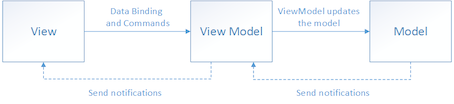
\includegraphics{images/mvvm-pattern.png}
    \caption{MVVM Pattern; Source \autocite{stonis2022mvvm}}
\end{figure}

Based on the diagram provided above and the documentation \autocite{stonis2022mvvm}, it can be inferred:
\begin{enumerate}
    \item The Model:\newline
    The Model holds the data and the business entities or objects. It represents the data access and manipulation logic, data validation, and persistence. The Model does not have any direct link to the View
    \item View: \newline
    The View is responsible for the user interface and visual presentation. The View does not contain any business logic.
    \item ViewModel: \newline
    the ViewModel is the crucial link between the Model and View which also holds the business logic. It provides the data and behavior that the View requires to display and interact with the data. The ViewModel exposes properties and commands that the View can bind to, allowing it to display the data and react to user interactions. 
\end{enumerate}



\chapter{Requirement Analysis}
This chapter includes analysis of the requirements of the system based on the problem statement described in the previous chapter. Furthermore, the main goal of the software as well as other specifications will be analyzed.

\section{Goal}
The goal of this research project is to build a functional prototype of a mobile application that monitors users' health and activity by observing users' heart rate. To observe one's heart rate, the application will be establish connection to a heart rate sensor via bluetooth low energy.
With the help of bluetooth low energy connection, the sensor is able to broadcast heart rate data to the application while consuming minimal energy.
The retrieved data will be stored in local database instead of cloud services or wearable devices to ensure data privacy. The user will also be given full control over their data, allowing them to modify or delete their data according to their will at anytime.
The retrieved data can be accessed later for visualization purposes as long as it is available. Furthermore, the application should be able to calculate users' energy expenditure during their exercise based on their heart rate, age, gender, weight, duration of exercise.

\section{State of the Art}
Health monitoring using wearable devices has gained immense popularity, enabling individuals to conveniently monitor their health and fitness. Bluetooth low energy (BLE) plays an important role in establishing connection between wearable device, which acts as a sensor, and the application. 
BLE offers real-time data exchange while consuming low power, which allows for long-term deployment without the need of frequent battery change. \cite{strey2013ble}
Existing health and activity monitor applications utilizing BLE offer a range of features and functionalities such as heart rate, calories burned, sleep patterns.

Nevertheless, as mentioned earlier, the challenges remain in maintaining a straightforward application and ensuring users' privacy. The aim in this research project is to explore the possibilities of improving health and wellbeing of the user by providing real-time data on their heart rate while providing users full control over their own data.
By addressing these challenges, this research project intends to develop a prototype of a more user- and privacy-friendly health activity monitor application using BLE.
\newpage

\section{Requirements}
\label{chap:requirements}
In this chapter, the requirements of the application is listed by identifying and analyzing the use cases from the research project's goals and priorities.

\subsection{Use Cases}
A use case diagram is created to provide a clearer understanding of how the system works and the various usage scenarios. It offers a clear and straightforward visualization that aligns with the goal of the research project.
\begin{figure}[H]
    \centering
    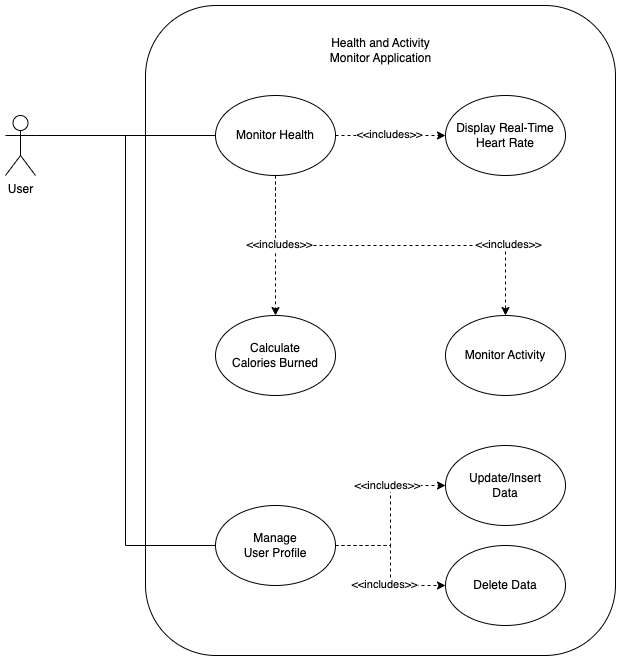
\includegraphics[width=1\textwidth]{diagrams/usecase.drawio.png}
    \caption{Use case diagram of the health and activity monitor application}
    \label{fig:use_cases}
\end{figure}
\newpage
The use case diagram provides visual presentation of the primary system functionalities and identifies the actor that interacts with the system.
The system includes several use cases to provide a comprehensive experience for monitoring health and activity while ensuring user's data privacy.

The primary use case, "Monitor Health", allows users to track important health indicators such as heart rate, calories burned, and current activity. It consists of three sub-use cases: "Display Real-Time Heart Rate", which shows the user's live heart rate on the application's interface; "Calculate Calories Burned", which calculates the number of calories burned in an exercise based on the user's heart rate;  "Monitor Activity", which observes the user's ongoing physical activity. In addition, the system includes "Manage User Profile" use case, which handles user profile management and data manipulation. Users can update or insert or delete data anytime using the respective sub-use cases. By integrating these use cases, the system effectively monitor health metrics and allows user to conveniently manage their data.

\subsection{User Stories}
According to the use cases visualized on \autoref{fig:use_cases}, the following user stories can be determined:

\begin{itemize}[label={},leftmargin=*]
    \item \textbf{Display Real-Time Heart Rate}
      \begin{itemize}[label={},leftmargin=*]
        \item As a health-minded user, I want the application to show my live heart rate so that I can monitor my cardiovascular activity.
      \end{itemize}

    \item \textbf{Track and Monitor Current Activity}
      \begin{itemize}[label={},leftmargin=*]
        \item As an physically active individuals, I want the application to track and display my current activity so that I can keep track of my progress and make adjustments to my physical activities.
      \end{itemize}

    \item \textbf{Calculate Calories Burned}
      \begin{itemize}[label={},leftmargin=*]
        \item As a fitness enthusiast, I want the application to calculate and display the number of calories burned based in my exercises. This allows me to keep track of my progress and make adjustments to my exercises.
      \end{itemize}  

    \item \textbf{Profile Management}
      \begin{itemize}[label={},leftmargin=*]
        \item As a user of the application who is concerned about data privacy, I want to be able to manage my user profile easily. This includes updating or adding new information to my profile and create a new profile. I also want the ability to delete my data anytime. This allows me to have full control over my data.
      \end{itemize}
  \end{itemize}


\subsection{Application Quality Standard}
The evaluation of the system developed for this research project is guided by the core application quality standard outlined in Android Documentation \autocite{androidqualityguidelines}. These quality standards provide core foundation for assessing the quality of the application. To facilitate the evaluation a set of criteria is derived from the core application quality standard described outlined in Android Documentation \autocite{androidqualityguidelines}. The table below shows the criteria, along with the sub-characteristic as well as its relevance to the research project. These criteria will be reviewed during the evaluation process to assess the quality of the application developed in this research project.
\label{tab::qualitystandard}

\begin{longtable}{p{0.2\textwidth} p{0.1\textwidth} p{0.5\textwidth} p{0.2\textwidth}}

    \caption{Core application quality standard based on Android Documentation \autocite{androidqualityguidelines} and its importance}\\

        \hline
        \textbf{Area} & \textbf{ID} & \textbf{Description} & \textbf{Relevance} \\
        \hline
        Navigation & VX-N1 & The app supports standard Back button navigation and does not make use of any custom, on-screen "Back button" prompts. & less important \\
         & VX-N2 & The app supports gesture navigation for going back / going to the home screen. & less important \\
         & VX-N3 & The app correctly preserves and restores user or app state. & important \\
  
        UI and Graphics & VX-U1 & The app supports both landscape and portrait orientations (if possible) and folding / unfolding. & important \\
         & VX-U2 & The app uses the whole screen in both orientations and does not letterbox to account for orientation changes, including folding and unfolding. & not important \\
         & VX-U3 & The app correctly handles rapid transitions between display orientations and device folding / unfolding without rendering problems or losing state. & less important \\
  
        Visual quality & VX-V1 & The app displays graphics, text, images, and other UI elements without noticeable distortion, blurring, or pixelation. The app should use vector drawables where possible. & less important \\
         & VX-V2 & The app displays text and text blocks in an acceptable manner for each of the app's supported languages. & important \\
         & VX-V3 & The app's content, and all web contents referred to by the app, support dark theme. & not important \\
        Accessibility & VX-A1 & Touch targets should be at least 48dp in size. & less important \\
         & VX-A2 & The app's text and foreground content should maintain a high enough color contrast ratio with its background. & important \\
         & VX-A3 & Describe each UI element, except for TextView, using contentDescription. & not important \\
  
        Background Service & FN-B1 & The app avoids running unnecessarily long services in the background. To ensure the smooth running of the user's device, the system applies various restrictions on background services. & important\\

        Stability & PS-S1 & The app does not crash or block the UI thread causing ANR ("Android Not Responding") errors.  & very important\\

        Performance & PS-P1 & The app loads quickly or provides onscreen feedback to the user (a progress indicator or similar cue) if the app takes longer than two seconds to load. & important\\
        & PS-P2 & Apps should render frames every 16ms to achieve 60 frames per second. Developers can use the Profile HWUI rendering option in testing. If there are issues, tools are available to help diagnose slow rendering. & less important\\
        & PS-P3 & With StrictMode enabled (see StrictMode Testing, below), no red flashes (performance warnings from StrictMode) are visible when testing the app. Any red flashes indicate bad behaviors regarding storage, network access, or memory leaks.  & less important\\
        
        Permissions & SC-P1 & The app requests only the absolute minimum number of permissions that it needs to support its use case at hand. & important \\
        & SC-P2 & The app requests permission to access sensitive data (such as SMS, Call Log, or Location) or services that cost money (such as Dialer or SMS) only when directly related to the core use cases of the app. & important \\
        & SC-P3 & The app requests runtime permissions in context, when the functionality is requested, rather than upfront during app startup. & less important\\
        & SC-P4 & The app clearly conveys why certain permissions are needed or follows the recommended flow to explain why it needs a permission. &  important \\
        & SC-P5 & The app should gracefully degrade when users deny or revoke a permission. The app should not prevent the user from accessing the app altogether. & important\\
        
        Data \& Files & SC-DF1 & All sensitive data is stored in the app's internal storage. & important\\
         & SC-DF2 & No personal or sensitive user data is logged to the system log or an app-specific log. & important\\
         & SC-DF3 & The app does not use any non-resettable hardware IDs, such as the IMEI, for identification purposes. & less important\\

        
        \hline
\end{longtable}


\chapter{Conception}
This chapter describes the concept and design of the application based on the previously analyzed requirements. This chapter outlines the application's structure, functionalities, technologies, and patterns used to fulfill the listed requirements.

\section{System Architecture}
In this section, an architecture diagram is displayed to have a better understanding of the system architecture as well as its components.
\begin{figure}[H]
    \centering
    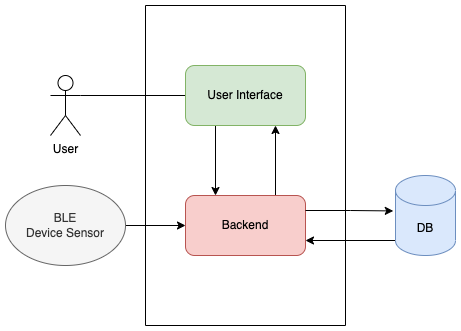
\includegraphics[width=1\textwidth]{diagrams/system-diagram.drawio.png}
    \caption{System architecture diagram}
    \label{fig:sys_diagram}
\end{figure}
\autoref{fig:sys_diagram} illustrates the components of the systems and the interaction between the components. Within the system, there are two components: the user interface and the backend which connects to a local database to store and manage data.
In addition, the device sensor is connected to the backend via bluetooth low energy and transmit the user's heart rate.
\section{Software Architecture}
This section serves as a guide to the high level structure of the application. It defines the key components as well as their relationship with each other.
Moreover, it describes the fundamental design patterns and architecture that define the application and its functionalities. 
The diagram presented below helps to gain better understanding of the application's architecture.
\begin{figure}[H]
    \centering
    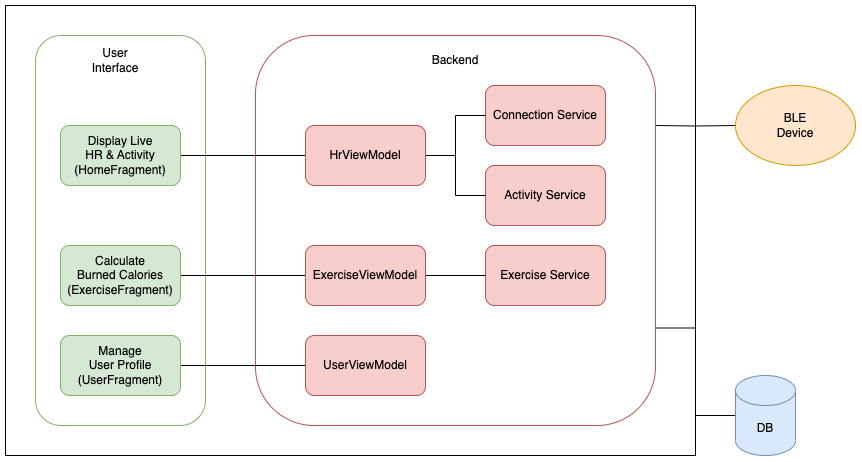
\includegraphics[width=1\textwidth]{diagrams/architecture-diagram.drawio.png}
    \caption{Software architecture diagram}
    \label{fig:soft_diagram}
\end{figure}
The project follows the Model-View-ViewModel (MVVM) architectural pattern. The user interface, which is responsible for displaying the features to the user, represents the \emph{view}. 
The \emph{model} is represented by the data and the business logic of the application, for instance, the entities and the functionalities such as live heart rate monitor, activity monitoring, exercise service, and user data management. 
The \emph{view model} facilitate the communications between the \emph{models} and the \emph{views} through which the \emph{views} can access and interact with the data and operations of the \emph{models}.

The user interface consists of three main components which extends \texttt{Fragment}\footnote{Based on The Official Android Documentation, a Fragment represents a reusable portion of your app's UI. A fragment defines and manages its own layout, has its own lifecycle, and can handle its own input events. \autocite{android-fragments}}. 
The \texttt{HomeFragment} displays real-time heart rate data and the activity monitor. It serves as the initial entry point for the users as they log in to the application. As it shows live heart rate data and activity, it holds a connection to the \texttt{HrViewModel}.
The \texttt{ExerciseFragment} presents the number of calories burned in an exercise based on the user's heart rate. It maintains a connection with the \texttt{ExerciseViewModel}. Lastly, the \texttt{UserFragment}, which is connected to the \texttt{UserViewModel}, displays the user's data and provide the necessary UI components to support data management.

The backend is in charge of the core functionalities of the application, which involve establishing a connection to the database.
As one of the core components, the \texttt{ConnectionService} maintains the connection between the BLE device and the application. It actively listens to the heart rate data being broadcasted by the BLE device. 
The \texttt{ActivityService} determines the current activity status based on the user's heart rate and age. 
On the other hand, the \texttt{ExerciseService} tracks the user's energy expenditure during training based on the user's heart rate and physical measurements such as weight, age, and gender. Both the \texttt{ExerciseService} and \texttt{ActivityService} subscribe to an event, where the heart rate data is published by the \texttt{ConnectionService}. This enables the services to receive the heart rate data seamlessly and process it accordingly.
Lastly, the \texttt{UserViewModel} is responsible for the management of the user's data and facilitates CRUD operations related to the user's data.

\section{Technologies}
\label{chap:tech}
This section provides an overview of the key technologies required to develop the application. 
The goal of this phase is to find the most suitable technologies based on the goal of this project and preferences of the writer. 
Android with Kotlin is chosen as the development platform for this project due to its widespread popularity and compatibility with the Model-View-ViewModel architectural pattern. Additionally, Android offers a wide range of development tools and resources, making it suitable for this project.

\subsection{User Interface}
As the main development platform for this project is Android Kotlin, the user interface is designed and implemented using a combination of Kotlin and XML with the help of Material Design\footnote{\emph{Material Design} is a design language developed by Google. Homepage: \url{https://m2.material.io/develop/android}}.
Implementing a graph to display live heart rate data can be advantageous to the user. Therefore, for smooth and appealing visualization, MPAndroidChart\footnote{\emph{MPAndroidChart} is a chart library for Android, designed for generating interactive and dynamic charts. Github repository: \url{https://github.com/PhilJay/MPAndroidChart}} is used to help with the graph implementation.
\subsection{Backend Infrastructure}
As mentioned before, the backend of the application is developed using Kotlin with Android Jetpack\footnote{\emph{Jetpack} is a suite of libraries, tools, and guidance to help developers write apps easier. URL: \url{https://developer.android.com/jetpack}} due to its compatibility with the MVVM architecture. 
Furthermore, Kotlin provides pre-defined classes such as the \emph{Service}\footnote{Based on The Official Android Documentation, \emph{Service} is an application component that can perform long-running operations in the background.\autocite{android-services}} class, which enables smooth execution of long running task. In the scope of this project, \emph{Service} class is especially useful to implement the \texttt{ConnectionService} and \texttt{ExerciseService}.

\subsection{Database}
A database is required to store and manage data. In the context of this project, ROOM\footnote{\emph{ROOM} is a persistence library that provides an abstraction layer over SQLite to allow for more robust database access while harnessing the full power of SQLite. URL: \url{https://developer.android.com/jetpack/androidx/releases/room}} database, which is built on top of SQLite\footnote{\emph{SQLite} is a C-language library that implements a small, fast, self-contained, high-reliability, full-featured, SQL database engine. Homepage: \url{https://www.sqlite.org/index.html}} has been selected as the application's database.

\subsection{BLE Sensor Device}
Once all the technologies required to develop the application have been decided, the next step is to select a suitable heart-rate sensor device. Considering factors like accuracy, performance, and affordability, Polar H9\footnote{\emph{Polar H9} is a heart rate sensor made by Polar. Homepage: \url{https://www.polar.com/en/sensors/h9-heart-rate-sensor}} is chosen as the preferred device due to its affordability and reputation for providing reliable heart-rate measurements and long battery life.
\section{Software Design}
This section outlines a strategy to transform the requirements of the application defined in \autoref{chap:requirements} into a well-defined and structured application.
As the project follows the MVVM architectural pattern, the application is divided into three components: \emph{model}, \emph{view}, \emph{view model}. 

\subsection{Model}
\label{chap:model_design}
The \emph{model} represents the business logic to solve the problems listed as the requirements of the systems. Once the use cases outlined in \autoref{chap:requirements} are analyzed, the functions of each system components can be determined and then a sequence of operations can be created for each specific use case.
To gain a better overview and understanding of the entities inside the system, a diagram is created.
\begin{figure}[H]
    \centering
    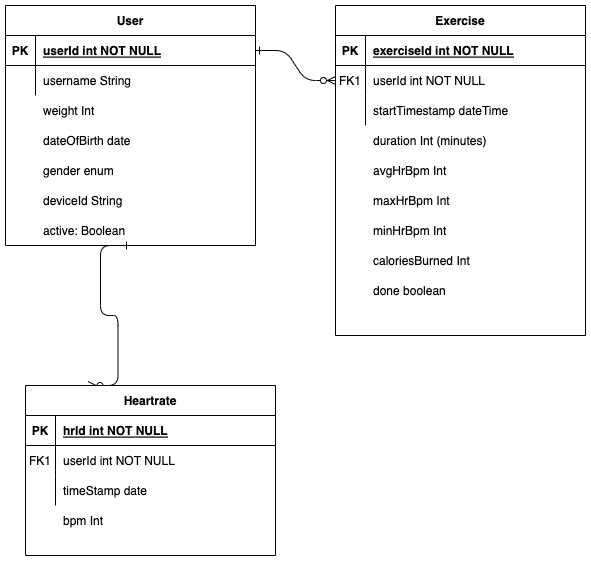
\includegraphics[width=0.8\textwidth]{diagrams/ham-entity.drawio.png}
    \caption{Entity class diagram}
    \label{fig:entity_diagram}
\end{figure}
{{\ttfamily \hyphenchar\the\font=`\-}
\autoref{fig:entity_diagram} visualizes the main entities and its relationship with each other inside the system. As illustrated by the diagram, the main entities in the system consist of \texttt{User}, \texttt{Exercise}, \texttt{Heartrate}. 
Each \texttt{User} within the system has one to many relationship with both \texttt{Heartrate} and \texttt{Exercise} entities. These relationships represent the connection between a \texttt{User} and their corresponding \texttt{Heartrate} and \texttt{Exercise} records. 
Once the entities have been defined, the system's functionalities can now be discussed based on the identified use cases.
\par}


\subsubsection{Heart Rate Monitor}
\label{chap:hr_monitor_design}
A system sequence can now be defined as a result of analyzing the following user story:
\begin{quotation}
    \enquote{As a health-oriented user, I want to monitor my cardiovascular activity.} 
\end{quotation}

\begin{figure}[H]
    \centering
    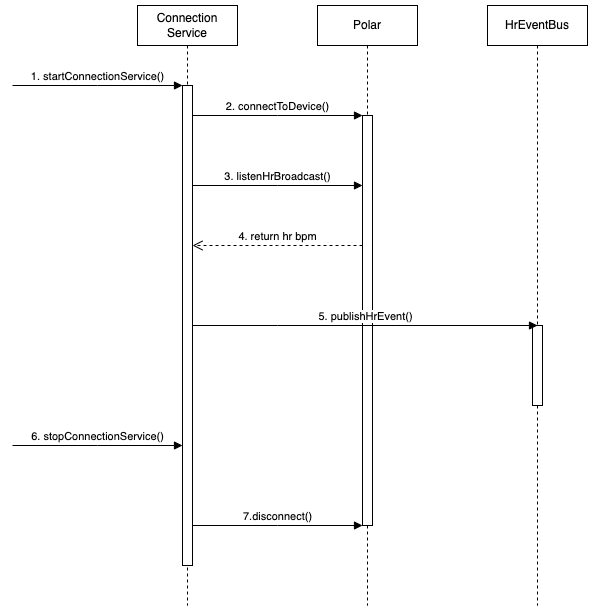
\includegraphics[width=0.9\textwidth]{diagrams/connection-service-onStart.drawio.png}
    \caption{Connection service sequence diagram}
    \label{fig:connection_diagram}
\end{figure}
Since one of the requirements is to monitor real-time heart rate, it is mandatory to establish connection to the heart rate sensor and handle the broadcasted heart rate data. The user should have a way to easily connect and disconnect from the device as desired.
The following sequence is visualized in \autoref{fig:connection_diagram} and it will be executed as a way to maintain connection to the BLE heart rate sensor and retrieve the heart rate data.
\begin{enumerate}
    \item A request to start the \texttt{ConnectionService} is received.
    \item The service initiates a bluetooth low energy connection to the heart rate sensor device.
    \item After the connection has been established, the \texttt{ConnectionService} listens to the heart rate data broadcasted by the heart rate sensor device.
    \item The heart rate sensor broadcasts heart rate data.
    \item The service publishes an event containing the received heart rate data to the \texttt{HrEventBus}.
    \item A request to stop the \texttt{ConnectionService} is received.
    \item The service stops the connection with the heart rate sensor device.
\end{enumerate}

\subsubsection{Activity Monitor}
\label{chap:activity_monitor_design}
Based on the analysis of the following user story, a system sequence that outlines the sequence of actions and interactions within the system can now be established.
\begin{quotation}
    \enquote{As an physically active individuals, I want to track my current activity so that I can make adjustments to my physical activities.} 
\end{quotation}

\begin{figure}[H]
    \centering
    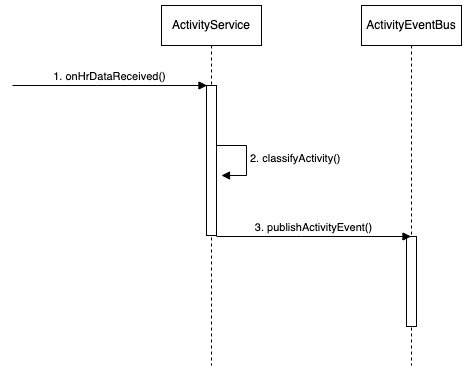
\includegraphics[width=0.8\textwidth]{diagrams/activity-monitor-seq.drawio.png}
    \caption{Activity service sequence diagram}
    \label{fig:activity_diagram}
\end{figure}

The following sequence in \autoref{fig:activity_diagram} illustrates the steps in monitoring the user's activity, which is one of the key use cases in the system:
\begin{enumerate}
    \item The \texttt{ActivityService} actively listens to the heart rate event broadcasted by the \texttt{ConnectionService} to the \texttt{HrEventBus}.
    \item Every time a heart rate event received, the \texttt{ActivityService} classifies the user's current activity based on the user's current heart rate by using the formula mentioned in \autoref{chap:activity_intensity}
    \item Once the heart rate is classified, the service publishes an event containing the current activity.
\end{enumerate}

\subsubsection{Calculate Energy Expenditure}
\label{chap:burnedcalories_design}
Given that one of the requirements defined in the use cases of the system is to calculate burned calories or energy expenditure, it is necessary to implement a feature that enables the calculation of energy expenditure. 
Based on the formula mentioned in \autoref{chap:energy_expenditure}, it is required to specify the duration during which the calculation will be performed. 
To facilitate this, it is recommended to create a record of exercise. The exercise should hold the attributes needed for the calculation of the energy expenditure, for instance, the duration of the exercise and the average heart rate bpm.
Prior to initiating an exercise, it is necessary for the user to establish a connection with the heart rate sensor. This ensures the availability of real-time heart rate data, which is vital for accurate energy expenditure calculations during the exercise.

A system sequence can now be defined as a result of analyzing the following user story:
\begin{quotation}
    \enquote{As a fitness enthusiast, I want to know the number of calories burned in my exercises. This allows me to keep track of my progress and make adjustments to my exercises.} 
\end{quotation}

The following sequence is illustrated in \autoref{fig:start_exercise_diagram} and it is executed as a way to track the current exercise and calculate the energy expenditure:
\begin{enumerate}
    \item A request to start the exercise is received.
    \item The \texttt{ExerciseService} retrieves the active exercise from the repository, which is created and set active by the \texttt{ExerciseViewModel} when the user starts the exercise
    \item active exercise is returned
    \item The \texttt{ExerciseService} actively listens to the heart rate event broadcasted by the \texttt{ConnectionService}.
    \item Heart rate event is retrieved.
    \item The \texttt{ExerciseService} processes active exercise. In this process, the attributes within the exercise such as average bpm and burned calories are calculated.
    \item The \texttt{ExerciseService} publishes an event containing the processed exercise.
    \item The processed exercise is persisted to the database.
    \item The persisted exercise is returned.
    \item A request to stop the exercise is received.
    \item The active exercise is marked as done.
    \item The \texttt{ExerciseService} publishes an event containing the completed exercise.
    \item The completed exercise is persisted to the database.
    \item The persisted exercise is returned.
\end{enumerate}

\begin{figure}[H]
    \centering
    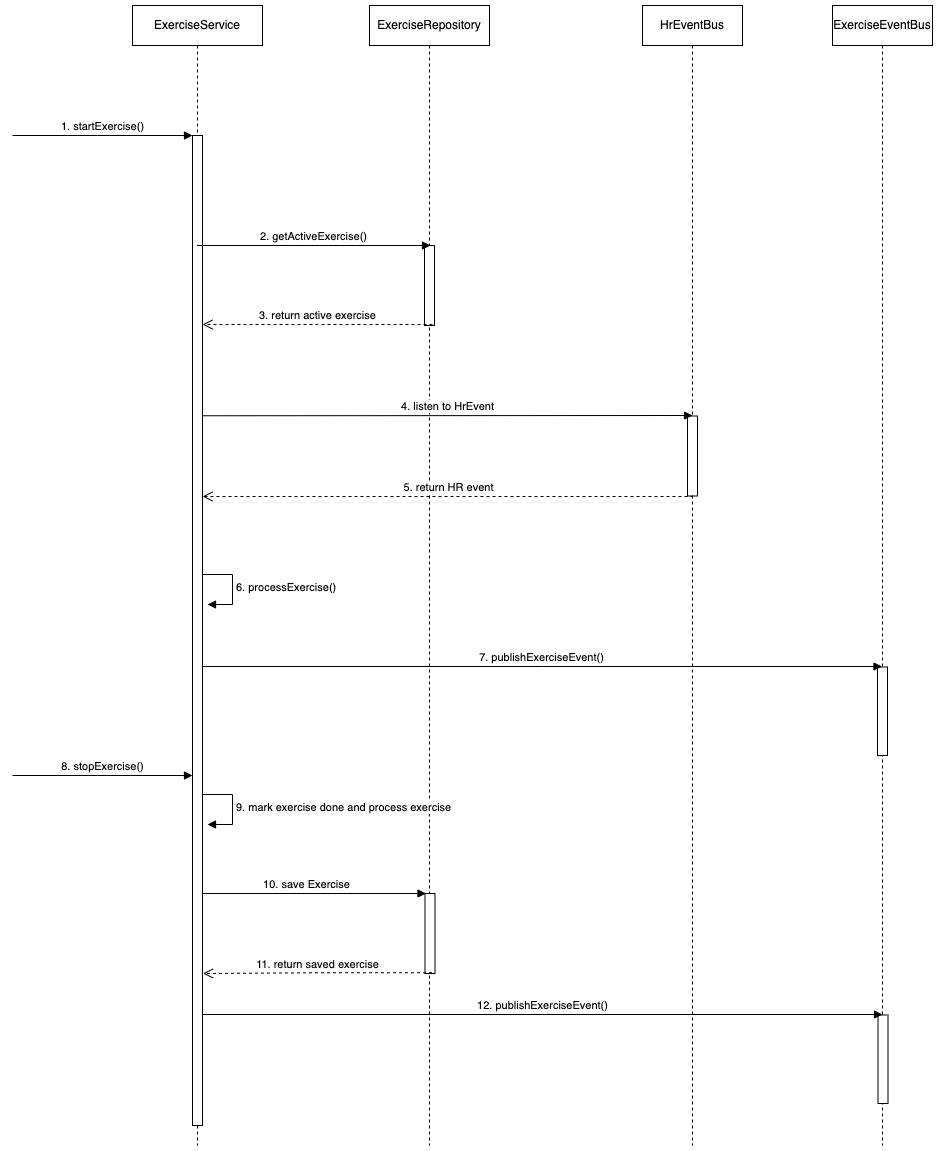
\includegraphics[width=1\textwidth]{diagrams/exercise-service-start.drawio.png}
    \caption{Exercise service on start and stop exercise sequence diagram}
    \label{fig:start_exercise_diagram}
\end{figure}

\subsubsection{Event Bus}
As the \emph{services} need to communicate with each other, it is very advantageous to implement an event bus based on the observable pattern described in Design Patterns \autocite{gamma1995design}. 
It involves using an event bus as a central hub for publishing and subscribing to events. Components can publish events to the bus without needing to know the receivers, and they can subscribe to specific types of events without knowing the publishers \autocite{turan2017}.
In the context of this project, there are three major event bus: \texttt{HrEventBus}, which handles events related to heart rate data; \texttt{ActivityEventBus}, responsible for managing events related to activity status; and lastly \texttt{ExerciseEventBus}, dedicated to handling exercise events.

\subsubsection{Profile Management}
According to the defined use cases in \autoref{chap:use_case}, it is essential to develop a functionality that enables users to manage their personal data. This functionality includes creating a new user profile, allowing users to modify their existing data, and lastly providing the users the capability to permanently delete their own data. These features will be implemented at the \emph{view model} level.
It will be discussed on \autoref{chap:viewmodel_design}




\subsection{ViewModel}
\label{chap:viewmodel_design}
\subsection{View}
The \emph{view}, which serves as the user interface, provides an interface for the user to interact with the application. The \emph{view} will be implemented as a graphical user interface (GUI) to enhance the user experience. 
It is responsible for displaying the pre-defined functionalities in \autoref{chap:model_design}, allowing users to easily navigate and use the features provided by the application. 
Several mock-ups have been designed using the UI design tool UIzard\footnote{UIzard is a UI design tool used for designing wireframes, mockups, and prototypes. Homepage: \url{https://uizard.io/}} to provide a clearer visualization of the layout of the user interface.

\subsubsection{HomeFragment}
The \emph{HomeFragment} serves as the main screen of the application, providing an overview of the user's health and activity-related functionalities defined in \autoref{chap:hr_monitor_design}. This \emph{view} consists of various components, including real-time heart rate display and activity monitor.
The real-time heart rate display dynamically shows the user's live heart rate, allowing them to track their cardiovascular activity. Additionally, it features a dynamic graph that visualizes the user's heart rate history, which enables them to track their heart rate patterns over time.
The activity monitor informs the user's current activity intensity based on their current heart rate, which enables them to track their activity intensity and adjust their current activity intensity according to their needs. As mentioned in \autoref{chap:activity_intensity}, the intensity levels range from very light, light, moderate, hard, and very hard.

\begin{figure}[H]
    \centering
    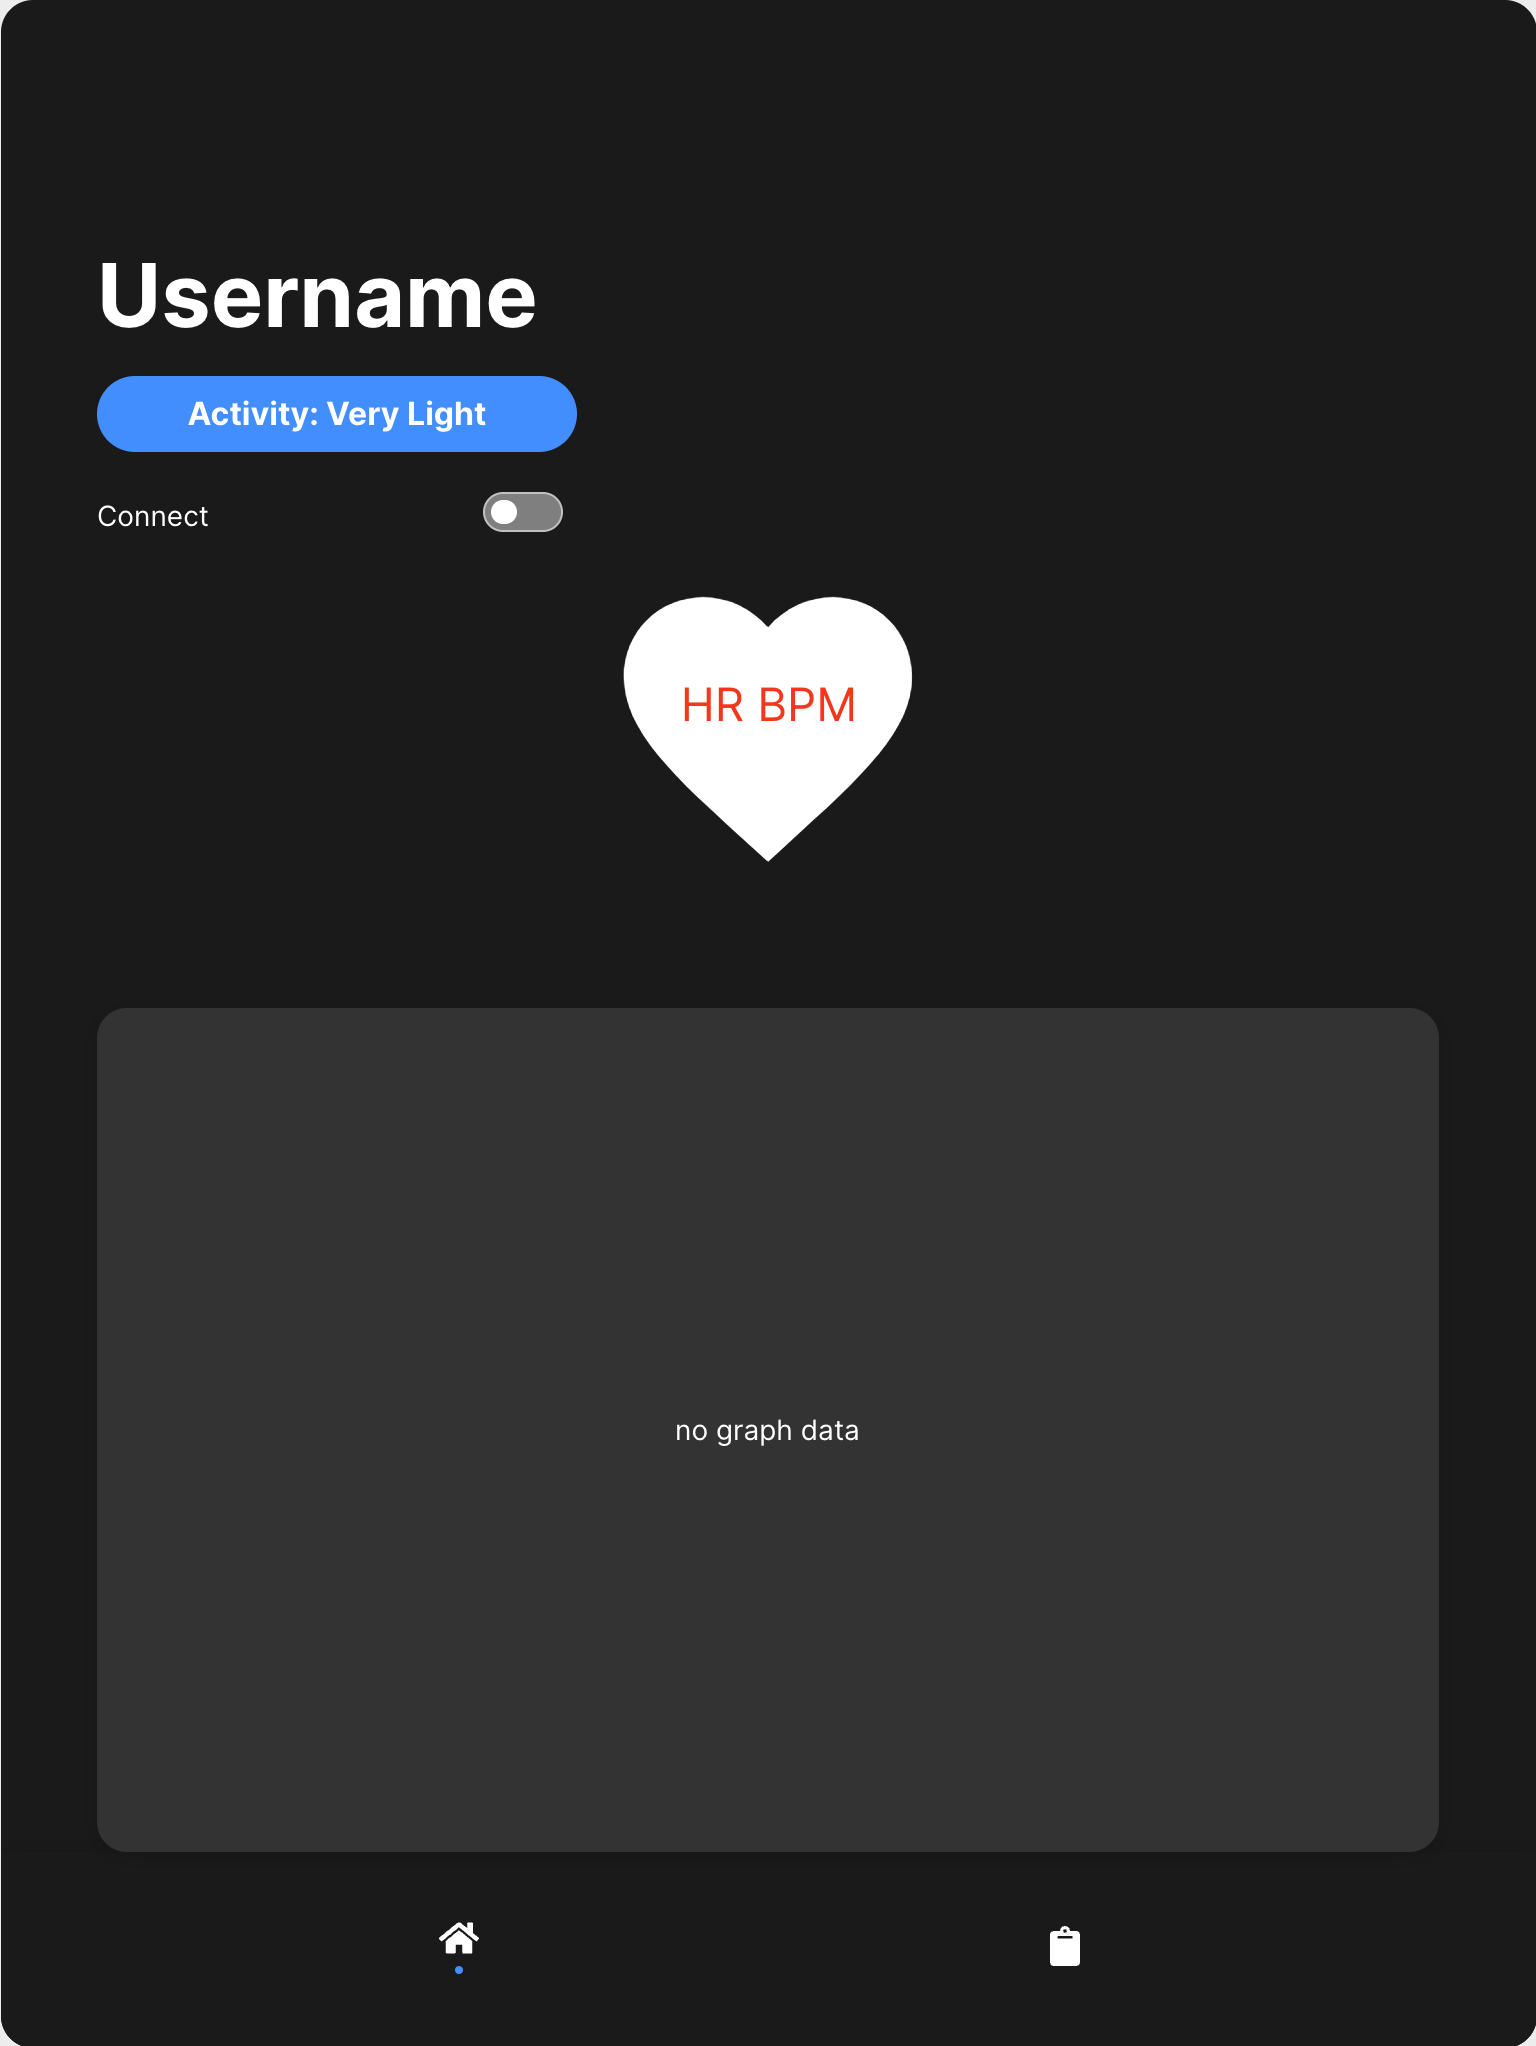
\includegraphics[width=0.75\textwidth]{images/home-fragment-mockup.png}
    \caption{HomeFragment mock-up}
    \label{fig:homefragment_mockup}
\end{figure}

As part of the real-time tracking and display of heart rate and current activity, the following sequence is executed:
\begin{enumerate}
    \item A switch is pressed to connect the application to the heart rate sensor.
    \item A request to start connection service is sent to the \emph{ConnectionServiceManager}.
    \item The \emph{ConnectionService} is started.
    \item \emph{HomeFragment} actively observes the heart rate live data from \emph{HrViewModel}.
    \item \emph{HomeFragment} actively observes the current activity live data from \emph{HrViewModel}.
    \item when the values from both the live data change, \emph{HomeFragment} is notified.
    \item \emph{HomeFragment} updates the UI according to the data changes.

\end{enumerate}

\begin{figure}[H]
    \centering
    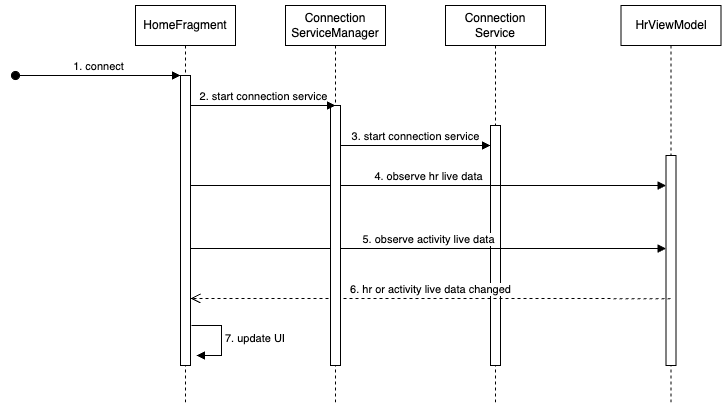
\includegraphics[width=1\textwidth]{diagrams/hr-broadcast-homefragment.drawio.png}
    \caption{HomeFragment sequence diagram}
    \label{fig:homefragment_diagram}
\end{figure}

As part of the requirement, the user interface must facilitate the functionality to stop the connection between the application and the heart rate sensor. Thus, the following sequence is needed:
\begin{enumerate}
    \item A switch is pressed to connect the application to the heart rate sensor.
    \item A request to start connection service is sent to the \emph{ConnectionServiceManager}.
    \item The \emph{ConnectionService} is started.
    \item \emph{HomeFragment} actively observes the heart rate live data from \emph{HrViewModel}.
    \item \emph{HomeFragment} actively observes the current activity live data from \emph{HrViewModel}.
    \item when the values from both the live data change, \emph{HomeFragment} is notified.
    \item \emph{HomeFragment} updates the UI according to the data changes.

\end{enumerate}

\begin{figure}[H]
    \centering
    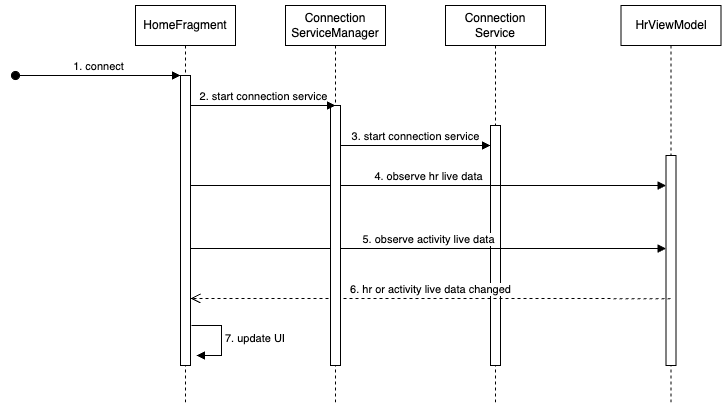
\includegraphics[width=1\textwidth]{diagrams/hr-broadcast-homefragment.drawio.png}
    \caption{HomeFragment sequence diagram}
    \label{fig:homefragment_diagram}
\end{figure}


\subsubsection{ExerciseFragment}
The \emph{ExerciseFragment} serves as the main component for presenting exercise details and displaying the calculation of energy expenditure. 
It shows an overview of the exercise, allowing users to access relevant information.








% \section{Features}

\chapter{Implementation}
This chapter focuses on the practical implementation of the software application based on the defined software design and requirements.
Moreover, it provides details on how the components, modules, and functionalities are implemented to develop the software system.

\section{Technologies}
The section describes the tools used in developing the system. 
As discussed in \autoref{chap:tech}, the system is mainly built using Kotlin supported by the following tools and technologies.

\subsection{Build Tool}
In this project, the default build tool for Kotlin, which is Gradle\footnote{\emph{Gradle} is a build automation tool used for  building, testing, and deploying software projects. Homepage: \url{https://gradle.org/}}, is used.
The Gradle Wrapper\footnote{\emph{Gradle Wrapper} is a script that runs Gradle commands without requiring an installation of Gradle on the local machine. URL: \url{https://docs.gradle.org/current/userguide/gradle_wrapper.html}} is naturally provided with Gradle. 
By using the script, gradle tasks such as build, test, and run can be easily executed.

\subsection{Code Style}
This project follows the guidelines and conventions enforced by lint\footnote{\emph{lint} is the default code style checker in Android Studio for Kotlin. URL: \url{https://developer.android.com/studio/write/lint}}.
Lint enforces coding standards and helps identify code style violations, ensuring a cleaner code. 
Additionally, the checkstyle runs automatically before each commit to ensure that the project follows to the coding conventions.

\subsection{PolarBleSDK}
The system uses the PolarBle software development kit (SDK)\footnote{\emph{PolarBleSDK} maintains bluetooth low energy connection for sensors made by Polar. Github repository: \url{https://github.com/polarofficial/polar-ble-sdk/}} to establish a and maintain a seamless connection between the heart rate sensor and the application.
Furthermore, the SDK provides tools and functionalities for data retrieval from the heart rate sensor.

\subsection{CI/CD}
In this project, Github Actions\footnote{\emph{Github Action} is a CI/CD platform available for repositories hosted in Github. Homepage: \url{https://github.com/features/actions}} is utilized as the CI/CD tool. 
The CI/CD pipeline is configured to be triggered automatically when there is a pull request to the main branch and when that branch is successfully merged. The configured CI/CD actions in this project is run test and build. 
This ensures that the code changes go through a standardized build and test process, maintaining the overall quality and stability of the project.

\subsection{Database}
In this project, Room is utilized as the database framework, which is based on SQLite. Room database is configured in kotlin as the following:
\begin{lstlisting}[caption={Room Database Configuration (Kotlin)}, label={list:database_config}]
@Database(entities = [User::class, Exercise::class, Heartrate::class], version = 4)
    @TypeConverters(DateTypeConverter::class, TimestampTypeConverter::class)
    abstract class HamDatabase: RoomDatabase() {
        abstract fun userDao(): UserDao
        abstract fun exerciseDao(): ExerciseDao
        abstract fun heartrateDao(): HeartrateDao
    
        companion object {
            @Volatile
            private var INSTANCE: HamDatabase? = null
    
            fun getInstance(context: Context): HamDatabase {
                synchronized(this) {
                    return INSTANCE ?: Room.databaseBuilder(
                        context.applicationContext,
                        HamDatabase::class.java,
                        DATABASE_NAME
                    )
                        .addMigrations(MIGRATION_2_3)
                        .fallbackToDestructiveMigration()
                        .build().also {
                        INSTANCE = it
                    }
                }
            }
    
            private val MIGRATION_2_3: Migration = object : Migration(2, 3) {
                override fun migrate(database: SupportSQLiteDatabase) {
                    database.execSQL("ALTER TABLE users ADD COLUMN active INTEGER NOT NULL DEFAULT 0")
                }
            }
        }
    }
          
\end{lstlisting}
The database schema consists of three entities: user, exercise, and heartrate, each representing a distinct data model.
These data access objects\footnote{\emph{Data Access Object (DAO)} serves as the main access point for interacting with the database. URL: \url{https://developer.android.com/training/data-storage/room/accessing-data}}: UserDao, ExerciseDao, heartrateDao, are configured, allowing interaction with the database. These DAOs define methods for querying data specific to each entities to the database.

In addition, two TypeConverters, namely DateTypeConverter and TimestampTypeConverter, are implemented to handle conversions between complex data types like Date and Timestamp to their corresponding storage representations in the database.

Room features an auto-migration functionality, where it automatically handles schema changes and data migration whenever a new version of the database is detected without the need of migration queries.
But in case of a conflict between the versions of the database, a Migration SQL query must be defined, ensuring seamless migration of the database.

\subsection{Dependency Injection}
To handle the dependency injection in this project, Hilt\footnote{\emph{Hilt} is a dependency injection library for Android that reduces the boilerplate of doing manual dependency injection in the project. Homepage: \url{https://developer.android.com/training/dependency-injection/hilt-android}} is used. 
It enables the injection of DAOs into their respective repositories and repositories into their corresponding ViewModels and other components that required to interact with the database. 
\begin{lstlisting}[caption={Dependency injection configuration (AppModule)}]
    @Singleton
    @Provides
    fun provideDatabase(
        @ApplicationContext app: Context
    ) = HamDatabase.getInstance(app)

    @Singleton
    @Provides
    fun provideUserDao(db: HamDatabase) = db.userDao()

    @Singleton
    @Provides
    fun provideExerciseDao(db: HamDatabase) = db.exerciseDao()

    @Singleton
    @Provides
    fun provideHeartrateDao(db: HamDatabase) = db.heartrateDao()
\end{lstlisting}
\subsection{Material Design}
To help developing a visually appealing and user-friendly interface, Material Design is used to develop the user interface as it contains several components that are suitable for the project. 
For instance, SwitchMaterial, MaterialButton, BottomNavigation.

\subsection{MPAndroidChart}
Additionally, MPAndroidChart helps generating an interactive and dynamic graph for visualizing heart rate history.
In the scope of this project, it is required to implement a line graph to visualize the heart rate data. 
Therefore, the LineChart\footnote{The implementation using \emph{LineChart} is discussed in \autoref{chap:view_impl}} in the MPAndroidChart is used to implement the heart rate data visualization.


\section{Model}
\label{chap:model_impl}
This chapter explains implementation details of the model defined in \autoref{chap:model_design}.

\subsection{Entities and Relationship}
\label{chap:objectmodel_impl}
In this subsection, the detailed implementation of the entities within the system and their relationships with each other will be discussed.

\subsubsection{User Entity}
The \verb;User; entity is responsible for storing and managing user data within the system.
It serves as a representation of an individual user and holds necessary data to support other functionalities.
Additionally, the \verb;User; entity has functions to calculate the user's age based on their date of birth and to estimate the maximum heart rate\footnote{\url{MAX_BPM_GLOBAL} is a global constant with an integer value of 220} using the formula mentioned in \autoref{chap:activity_intensity}.
\begin{lstlisting}[caption={User Entity (Kotlin)}]
@Entity(tableName = "users")
data class User(
    @PrimaryKey(autoGenerate = true) val userId: Long = 0,
    @ColumnInfo(name = "username") var username: String,
    @ColumnInfo(name = "weight") var weight: Int,
    @TypeConverters(DateTypeConverter::class)
    @ColumnInfo(name = "dateOfBirth") val dateOfBirth: Date,
    @ColumnInfo(name = "gender") var gender: Gender,
    @ColumnInfo(name = "deviceId") var deviceId: String,
    @ColumnInfo(name = "active") var active: Boolean = false
) {
    fun getAge(): Int {
        val currentDate = LocalDate.now()
        val dob = LocalDate.parse(dateOfBirth.toString())
        return Period.between(dob, currentDate).years
    }

    fun getMaxBpm(): Int {
        return (MAX_BPM_GLOBAL - 0.64*getAge()).toInt()
    }
}
\end{lstlisting}


\subsubsection{Exercise Entity}
The \verb;Exercise; entity manages information related to the user's exercises. 
This entity is responsible for tracking and recording user's exercise. Furthermore, the energy expenditure is also saved in this entity.
\begin{lstlisting}[caption={Exercise Entity (Kotlin)}]
@Entity(tableName = "exercises", foreignKeys = [
    ForeignKey(
        entity = User::class,
        parentColumns = ["userId"],
        childColumns = ["userId"],
        onDelete = ForeignKey.CASCADE
    )
])
data class Exercise(
    @PrimaryKey(autoGenerate = true) val exerciseId: Long = 0,
    @ColumnInfo(name = "userId", index = true) val userId: Long,
    @TypeConverters(DateTypeConverter::class)
    @ColumnInfo(name = "startTime") val startTime: Timestamp,
    @ColumnInfo(name = "duration") var duration: Int,
    @ColumnInfo(name = "averageHrBpm") var averageHrBpm: Int?,
    @ColumnInfo(name = "maxHrBpm") var maxHrBpm: Int?,
    @ColumnInfo(name = "minHrBpm") var minHrBpm: Int?,
    @ColumnInfo(name = "caloriesBurned") var caloriesBurned: Int?,
    @ColumnInfo(name = "done") var done: Boolean,
)
\end{lstlisting}


\subsubsection{Heartrate Entity}
The \verb;Heartrate; entity is responsible for storing heart rate information of users. 
This entity manages data that is valuable for monitoring users' cardiovascular health and exercise intensity.
\begin{lstlisting}[caption={Heartrate Entity (Kotlin)}]
@Entity(tableName = "heartrates", foreignKeys = [
    ForeignKey(
        entity = User::class,
        parentColumns = ["userId"],
        childColumns = ["userId"],
        onDelete = CASCADE
    )
])
data class Heartrate(
    @PrimaryKey(autoGenerate = true) val hrId: Long = 0,
    @ColumnInfo(name = "userId", index = true) val userId: Long,
    @ColumnInfo(name = "bpm") var bpm: Int,
    @TypeConverters(TimestampTypeConverter::class)
    @ColumnInfo(name = "timestamp") val timestamp: Timestamp,
)
\end{lstlisting}


\subsubsection{UserAndExercise Relationship}
The \verb;UserAndExercise; relationship establishes a one-to-many relationship between \verb;User; and \verb;Exercise;. 
This relationship allows \verb;User; to have multiple \verb;Exercise; associated with their profile. 
The relationship is defined with the "on delete cascade" constraint, ensuring that if a \verb;User; is deleted, all associated \verb;Exercise; are also deleted.

\subsubsection{UserAndHeartrate Relationship}
The \verb;UserAndHeartrate; relationship represents a one-to-many relationship between \verb;User; and \verb;Heartrate;. 
\verb;User; can have multiple \verb;Heartrate; entries associated with them. Similar to the The \verb;UserAndExercise; relationship, the "on delete cascade" constraint ensures that if a \verb;User; is deleted, their related \verb;Heartrate; data is also deleted.

\subsubsection{Activity Enum}
The \verb;Activity; enum is a predefined set of values that represents different levels of activity intensity. 
It provides a standardized way to categorize the intensity of physical activities based on the percentage of the user's maximum heart rate. 
The percentage intensity values mentioned in \autoref{chap:activity_intensity} are mapped to the activity enum, supporting \verb;ActivityService; to classify activity intensity level.


\subsection{Services}
This subsection provides the details of the implementation of the services within the system.

\subsubsection{Connection Service}
The implementation of the \verb;ConnectionService; follows the concept outlined in \autoref{chap:hr_monitor_design}. It focuses on establishing a connection with the heart rate sensor and listening to the heart rate data broadcasted by the heart rate sensor. 
It is implemented as a \verb;Service; class\footnote{A \emph{Service} is an application component that can perform long-running operations in the background. URL: \url{https://developer.android.com/guide/components/services}}, allowing it to run in the background even when the application is not in the foreground.

The lifecycle of the \verb;ConnectionService; is managed by \verb;ConnectionServiceManager;, which handles the start and stop operations. 
\texttt{ConnectionServiceManager} sends the active user's device id, attaching it to the \texttt{Intent}\footnote{\emph{Intent} is used to start, stop, and communicate with \emph{Service}. URL: \url{https://developer.android.com/reference/android/content/Intent}} used to initiate the \texttt{ConnectionService},
as the device id is required to start a connection to the heart rate sensor.
When the service is started, it automatically initiates the connection with the heart rate sensor.
\begin{lstlisting}[caption={Function to start ConnectionService (Kotlin - ConnectionServiceManager)}]
fun startConnectionService(context: Context, activeUser: User) {
    try {
        val serviceIntent = Intent(context, ConnectionService::class.java)
        serviceIntent.putExtra("deviceId", activeUser.deviceId)
        context.startForegroundService(serviceIntent)
        Log.d(HomeFragment.TAG, "started hr streaming")
    } catch (e: Exception) {
        Log.e(HomeFragment.TAG, e.message.toString())
    }
}
\end{lstlisting}

To establish the connection with the heart rate sensor, the \verb;ConnectionService; utilizes the PolarBleSdk library.
\begin{lstlisting}[caption={Function to initiate connection to heart rate sensor (Kotlin - ConnectionService)}]
private fun connectPolar(polarId: String) {
    polarBleApi.run {
        setApiLogger { s: String? -> Log.d(TAG, "CONNECTION_SERVICE LOGGER $s") }

        deviceConnected = try {
            connectToDevice(polarId)
            Log.d(TAG, "connected to $polarId")
            true
        } catch (polarInvalidArgument: PolarInvalidArgument) {
            Log.e(TAG, "Failed to connect. Reason $polarInvalidArgument ")
            false
        }

        setAutomaticReconnection(true)
    }
}
\end{lstlisting}

Once the connection to the heart rate sensor is established, \verb;ConnectionService; listens to the broadcasted heart rate data and publishes the data to \verb;HrEventBus;.
This allows other components of the system, such as the \verb;HrViewModel;, to subscribe to the \verb;HrEventBus; and receive real-time heart rate updates. 
\begin{lstlisting}[caption={Heart rate data broadcast listener (Kotlin - ConnectionService)}]
polarBleApi.startListenForPolarHrBroadcasts(null)
    .subscribe(
        { polarBroadcastData: PolarHrBroadcastData ->
            Log.d(TAG, "HR BROADCAST ${polarBroadcastData.polarDeviceInfo.deviceId} HR: ${polarBroadcastData.hr} batt: ${polarBroadcastData.batteryStatus}")
            onHrReceived(polarBroadcastData.hr)
            onBatteryReceived(polarBroadcastData.batteryStatus)
        },
        { error: Throwable ->
            Log.e(TAG, "Broadcast listener failed. Reason $error")
        },
        { Log.d(TAG, "complete") }
)
\end{lstlisting}

On the other hand, when the service is stopped by the \verb;ConnectionServiceManager;, the connection is gracefully terminated and the service will be stopped.

\subsubsection{Activity Service}
The \verb;ActivityService; is implemented based on \autoref{chap:activity_monitor_design}.
First, it listens to the \verb;HrEventBus;, which receives real-time heart rate data from the \verb;ConnectionService;. 
By subscribing to the \verb;HrEventBus;, the \verb;ActivityService; receives the latest heart rate data.
Every time heart rate data is received, this service determines the user's current activity based \autoref{chap:activity_intensity}.
\begin{lstlisting}[caption={Activity classifier (Kotlin - ActivityService)}]
private fun activityClassifier(bpm: Int, user: User) : Activity {
    val maxBpm = user.getMaxBpm()
    val veryLightBpm = maxBpm * Activity.VERY_LIGHT.intensity
    val lightBpm = maxBpm * Activity.LIGHT.intensity
    val moderateBpm = maxBpm * Activity.MODERATE.intensity
    val hardBpm = maxBpm * Activity.HARD.intensity
    val veryHardBpm = maxBpm * Activity.VERY_HARD.intensity

    return when (bpm) {
        in 0 until veryLightBpm.toInt() -> Activity.VERY_LIGHT
        in veryLightBpm.toInt() until lightBpm.toInt() -> Activity.LIGHT
        in lightBpm.toInt() until moderateBpm.toInt() -> Activity.MODERATE
        in moderateBpm.toInt() until hardBpm.toInt() -> Activity.HARD
        in hardBpm.toInt() until veryHardBpm.toInt() -> Activity.VERY_HARD
        else -> Activity.VERY_HARD
    }

}
\end{lstlisting}

Once the service classified the activity, the result will be published to \verb;ActivityEventBus;, allowing other components such as \verb;HrViewModel; to subscribe and receive the results.

\subsubsection{Exercise Service}
The implementation of this service follows the design described in \autoref{chap:burnedcalories_design}.
It records exercises done by the users and calculate the energy expenditure in that exercise.

Similar to the \verb;ConnectionService;, the lifecycle of the \verb;ExerciseService; is managed by another class named \verb;ExerciseServiceManager;, which handles the start and stop operations. 
When the service starts, it finds an active exercise and active user within the database. 
\begin{lstlisting}[caption={On ExerciseService started (Kotlin - ExerciseService)}]
    activeExercise = exerciseRepository.getActiveExercise()
    setUser(activeExercise.userId) // this is a wrapper function to find and set active user in the service level
\end{lstlisting}

For the calculation of burned calories, \verb;ExerciseService; needs the user's heart rate, To retrieve the actual heart rate data, it actively listens to \verb;HeartrateEvent; published to \verb;HeartrateEventBus;.
Every time heart rate event is received, \verb;ExerciseService; adds the heart rate bpm into a collection of \verb;Int; and updates the active exercise. The update process includes burned calories calculation based on \autoref{chap:energy_expenditure}. 
\begin{lstlisting}[caption={Process active exercise snippet (Kotlin - ExerciseService)}]
    listOfHr.add(bpm)

    activeExercise.averageHrBpm = listOfHr.average().toInt()
    activeExercise.maxHrBpm = listOfHr.maxOrNull()
    activeExercise.minHrBpm = listOfHr.minOrNull()
    activeExercise.duration = getSecondsBetweenTimestampAndNow(activeExercise.startTime)
    activeExercise.caloriesBurned = calculateCalories(activeExercise).toInt().coerceAtLeast(0)

    CoroutineScope(Dispatchers.IO).launch {
        exerciseRepository.upsertExercise(activeExercise)
    }
\end{lstlisting}

To prevent \url{ANR}\footnote{\emph{Android Not Responsive (ANR)} occurs when the main thread is blocked. URL: \url{https://developer.android.com/topic/performance/vitals/anr}}, the process to save the exercise to the database is run on a \emph{coroutine}\footnote{A \emph{coroutine} is a concurrency design pattern that you can use on Android to simplify code that executes asynchronously. URL: \url{https://developer.android.com/kotlin/coroutines}}.
Once the exercise is updated and saved, it will be published to \verb;ExerciseEventBus;, which allows \verb;ExerciseViewModel; to be up-to-date with the active exercise.

When the service is stopped by \verb;ExerciseServiceManager;, the service unsubscribes from the \verb;HeartrateEventBus;, mark the exercise as done, process the exercise and finally publish it to \verb;ExerciseEventBus;.
\begin{lstlisting}[caption={On exercise stopped snippet (Kotlin - ExerciseService)}]
    activeExercise.done = true
    HeartrateEventBus.unsubscribe(hrListener)
    processExerciseAndPublish()
\end{lstlisting}
\section{ViewModel}
This chapter explains implementation details of the view model designed in \autoref{chap:viewmodel_design}

\subsection{HrViewModel}
\label{chap:hrviewmodel_impl}
To support real-time updates of heart rate and activity data, the \verb;HrViewModel; uses \verb;LiveData; objects. These \verb;LiveData; objects include \verb;currentHrBpm;, \verb;currentActivity;, and \verb;currentHrList;.
The \verb;currentHrBpm; and \verb;currentActivity; contain the current heart rate bpm and activity intensity level respectively. On the other hand, the \verb;currentHrList; holds a list of \verb;Heartrate;.
\begin{lstlisting}[caption={LiveData implementation (HrViewModel)}]
    val currentHrBpm: MutableLiveData<Int> by lazy {
        MutableLiveData<Int>()
    }
    val currentActivity: MutableLiveData<String> by lazy {
        MutableLiveData<String>()
    }
    val currentHrList: MutableLiveData<List<Int>> by lazy {
        MutableLiveData<List<Int>>()
    }
\end{lstlisting}

In order to receive the heart rate and activity data, the \verb;HrViewModel; subscribes to the \verb;HrEventBus; and the \verb;ActivityEventBus;. 
When receiving data from the \verb;HrEventBus;, the \verb;HrViewModel; updates the value of \verb;currentHrBpm; and \verb;currentHrList;. 
Additionally, \verb;HrViewModel; saves the received heart rate data to the database and to prevent ANR, this process runs on a coroutine.
\begin{lstlisting}[caption={On heart rate event received (HrViewModel)}]
private fun onHrReceived(newHrBpm: Int) {
    Log.d(TAG, "new hr data received = $newHrBpm")
    currentHrBpm.value = newHrBpm
    val hr = Heartrate(
        userId = activeUser!!.userId,
        bpm = newHrBpm,
        timestamp = Timestamp(System.currentTimeMillis())
    )
    viewModelScope.launch {
        withContext(Dispatchers.IO) {
            hrRepository.save(hr)
        }
    }

    val temp = currentHrList.value?.toMutableList()
    temp?.add(newHrBpm)
    currentHrList.value = temp?.toList()
    Log.d(TAG, "hr list modified = ${currentHrList.value}")
}
\end{lstlisting}
When activity data from the \verb;ActivityEventBus; is received, the \verb;HrViewModel; updates the value of \verb;currentActivity;.
\begin{lstlisting}[caption={On activity event received (HrViewModel)}]
private fun onActivityReceived(newActivity: Activity) {
    currentActivity.value = newActivity.type
}
\end{lstlisting}

Additionally, the \verb;HrViewModel; retrieves the currently active user from the database upon initialization, and listens to \url{ActiveUserChangeEvent} to detect any changes in the active user.
When there are changes to the active user, the \verb;HrViewModel; updates the \verb;currentHrList; value with the current active user's list of heart rate data for graphing purposes.

\subsection{ExerciseViewModel}
\label{chap:exerciseviewmodel_impl}
{{\ttfamily \hyphenchar\the\font=`\-}
The \verb;ExerciseViewModel; maintains two live data objects: \texttt{currentExercise} and \texttt{currentExerciseList}, which hold the exercise information for the current session and the list of all exercises belonging to the active user, respectively. 
\par}

\begin{lstlisting}[caption={LiveData implementation (ExerciseViewModel)}]
    val currentExercise: MutableLiveData<Exercise> by lazy {
        MutableLiveData<Exercise>()
    }
    val currentExercisesList: MutableLiveData<List<Exercise>> by lazy {
        MutableLiveData<List<Exercise>>()
    }
\end{lstlisting}
The \verb;ExerciseViewModel; subscribes to the \verb;ExerciseEventBus; to receive updates on exercise events. Upon receiving data from the event bus, it updates the corresponding live data objects, ensuring that the view is always up to date with the latest exercise data.

{{\ttfamily \hyphenchar\the\font=`\-}
Similar to the \verb;HrViewModel;, the \verb;ExerciseViewModel; fetches the currently active user from the database upon initialization and actively observes \texttt{ActiveUserChangeEvent}.
The \verb;ExerciseViewModel; updates \verb;currentExercise; and \texttt{currentListExercise} accordingly when changes occur to the active user.
\par}

Additionally, the \verb;ExerciseViewModel; includes a logic to create an exercise with default values and save it to the database when the user starts a new exercise session. This logic ensures that the exercise is initialized with appropriate default values to support the start exercise functionality.
\begin{lstlisting}[caption={Create default exercise function (ExerciseViewModel)}]
fun createExerciseWithBasicFields(): Exercise {
    if (activeUser == null) {
        throw NoActiveUserException()
    }

    val exercise = Exercise(
        duration = 0,
        userId = activeUser!!.userId,
        averageHrBpm = 0,
        startTime = Timestamp(System.currentTimeMillis()),
        maxHrBpm = 0,
        minHrBpm = 0,
        caloriesBurned = 0,
        done = false
    )
    currentExercise.value = exercise

    viewModelScope.launch {
        exerciseRepository.upsertExercise(exercise)
    }

    return exercise
}
\end{lstlisting}

\subsection{UserViewModel}
\label{chap:userviewmodel_impl}
The \texttt{UserViewModel} manages two live data objects, for instance, \texttt{currentUser}, which contains the actual active user and \texttt{users}, which holds the list of all users in the database. 
Upon initialization, the \texttt{UserViewModel} sets the values of those live data by fetching it from the database.

The \texttt{UserViewModel} provides \texttt{setActiveUser} function to mark a user as active. When called, it updates the \texttt{currentUser} with the selected user and publishes \texttt{ActiveUserChangeEvent} to \texttt{ActiveEventBus}.
\begin{lstlisting}[caption={Set active user function snippet (UserViewModel)}]
    val au = userRepository.setActiveUser(userId)
    activeUser.postValue(au)
    publishActiveUser(au)
\end{lstlisting}

The \texttt{UserViewModel} implements \texttt{upsertUser} function. This function is responsible for updating an existing user or inserting a new user into the database. Once it is saved, it is marked automatically as the active user.
\begin{lstlisting}[caption={Save user function snippet (UserViewModel)}]
    val upserted = userRepository.upsertUser(user)
    setActiveUser(upserted.userId)
\end{lstlisting}

Lastly, the \texttt{UserViewModel} provides \texttt{upsertUser} function to delete active user completely from the system.
It checks if there are any running \texttt{ConnectionService} instances and also checks incomplete exercises. 
It only proceeds with the deletion if the validation is passed. Additionally, if there are other users remaining, the function automatically sets the latest user as the active user. Otherwise, null will be set as the active user.
\begin{lstlisting}[caption={Wrapper function for user deletion (UserViewModel)}]
private suspend fun deleteUser(user: User): Boolean {
    val activeExercise = userRepository.getActiveExerciseByUserId(user.userId)

    if (serviceRunningChecker.isServiceRunning(ConnectionService::class.java, getApplication())) {
        throw Exception("user has active hr sensor connection")
    }

    if (userRepository.getActiveExerciseByUserId(user.userId).isNotEmpty()) {
        throw Exception("user: ${user.userId} has active exercise: $activeExercise")
    }

    userRepository.deleteUser(user)
    return true
}
\end{lstlisting}

\begin{lstlisting}[caption={User deletion function (UserViewModel)}]
suspend fun deleteActiveUser() {
    var deleted = false
    activeUser.value?.let {
        try {
            deleted = deleteUser(it)
        } catch (e: Exception) {
            Log.e(TAG, e.message.toString())
        }
        if (deleted) {
            try {
                setActiveUser(userRepository.getUsers()[0].userId)
            } catch (e: Exception) {
                activeUser.postValue(null)
                publishActiveUser(null)
            }
        }
    }
}
\end{lstlisting}

\section{View}
\label{chap:view_impl}
The view in this project is implemented based on the concept designed in \autoref{chap:view_design}
\subsection{MainActivity}
The user interface displays several functionalities to fulfill the requirements of the system described in \autoref{chap:requirements}. To promote separation of concerns, the user interface is implemented in several \texttt{Fragment}, improving the code readability and maintainability.  
\texttt{MainActivity} serves as the container that binds the fragments together. To host and display different fragments based on the user's navigation, \texttt{FragmentContainerView}\footnote{\url{FragmentContainerView} is a customized Layout designed specifically for Fragments. URL: \url{https://developer.android.com/reference/androidx/fragment/app/FragmentContainerView}} is used.
The navigation between the fragments is controlled by the Android Navigation\footnote{\url{Navigation} is a framework provided by the Android Jetpack library that simplifies the implementation of navigation in an Android app. URL: \url{https://developer.android.com/guide/navigation}}, which is configured in a XML file. 
\begin{lstlisting}[caption={Navigation graph snippet for HomeFragment (XML - nav\_Graph)}, language=XML]
<fragment
    android:id="@+id/homeFragment"
    android:name="com.ham.activitymonitorapp.fragments.HomeFragment"
    android:label="HomeFragment"
    tools:layout="@layout/home_fragment">
    <action
        android:id="@+id/action_homeFragment_to_userFragment"
        app:destination="@id/userFragment" />
    <action
        android:id="@+id/action_homeFragment_to_exercisesFragment"
        app:destination="@id/exercisesFragment" />
</fragment>
\end{lstlisting}

The \texttt{MainActivity} provides a bottom navigation tool for users to navigate between the fragments. It is implented using the BottomNavigationView\footnote{\url{BottomNavigationView} represents a standard bottom navigation bar for application. URL: \url{https://developer.android.com/reference/com/google/android/material/bottomnavigation/BottomNavigationView}}.
\begin{figure}[H]
    \centering
    
\includegraphics[width=0.75\textwidth]{images/bottom-navbar.png}
    \caption{Screenshot of the bottom navbar}
    \label{fig:bottom_navbar}
\end{figure}

Additionally, \texttt{MainActivity} manages permission requests to ensure the necessary permissions are granted for the app's functionality. Specifically, it requests the \texttt{ACCESS\_COARSE\_LOCATION} permission.

\subsection{HomeFragment}
The implementation of \texttt{HomeFragment} includes several feature to fulfill the requirements of the system. 
Firstly, it provides a switch to control the connection to the heart rate sensor. This feature is disabled when there is no active user.

Moreover, the fragment displays the user's current heart rate (bpm) by observing the \texttt{currentHrBpm} LiveData from the \texttt{HrViewModel}. This ensures that the displayed heart rate is always up-to-date.
Additionally, the \texttt{HomeFragment} shows the user's current activity intensity level by observing the \texttt{currentActivity} LiveData also provided by the \texttt{HrViewModel}. 
\begin{lstlisting}[caption={Observers for currentActivity and currentHrBpm (HomeFragment)}]
    private fun observeHrData() {
        hrViewModel.currentHrBpm.observe(viewLifecycleOwner) { newHrData ->
            binding.heartRate.text = newHrData.toString()
        }
    }
    private fun observeActivity() {
        hrViewModel.currentActivity.observe(viewLifecycleOwner) { newActivity ->
            binding.activityMonitor.text = "Activity: $newActivity"
        }
    }
\end{lstlisting}

Furthermore, the fragment features an interactive graph that visualizes the user's heart rate data over time. 
The graph is controlled by another component called \texttt{GraphService} using the MPAndroidChart library, specifically the \texttt{LineChart} class.
The \texttt{GraphService} subscribes to the \texttt{HrEventBus}, which broadcasts heart rate data events. 
Whenever a heart rate data event is received, the \texttt{GraphService} updates the data set associated with the graph. 
This ensures that the graph is continuously updated with the latest heart rate data.
Additionally, the \texttt{GraphService} also reacts to changes in the active user. 
When the active user is changed, the \texttt{GraphService} generates a new graph based on the heart rate data of the new active user. 

Lastly, the \texttt{HomeFragment} observes the current active user and dynamically updates the user interface to display the current heart rate, activity level, and the graph.
\begin{figure}[H]
    \centering
    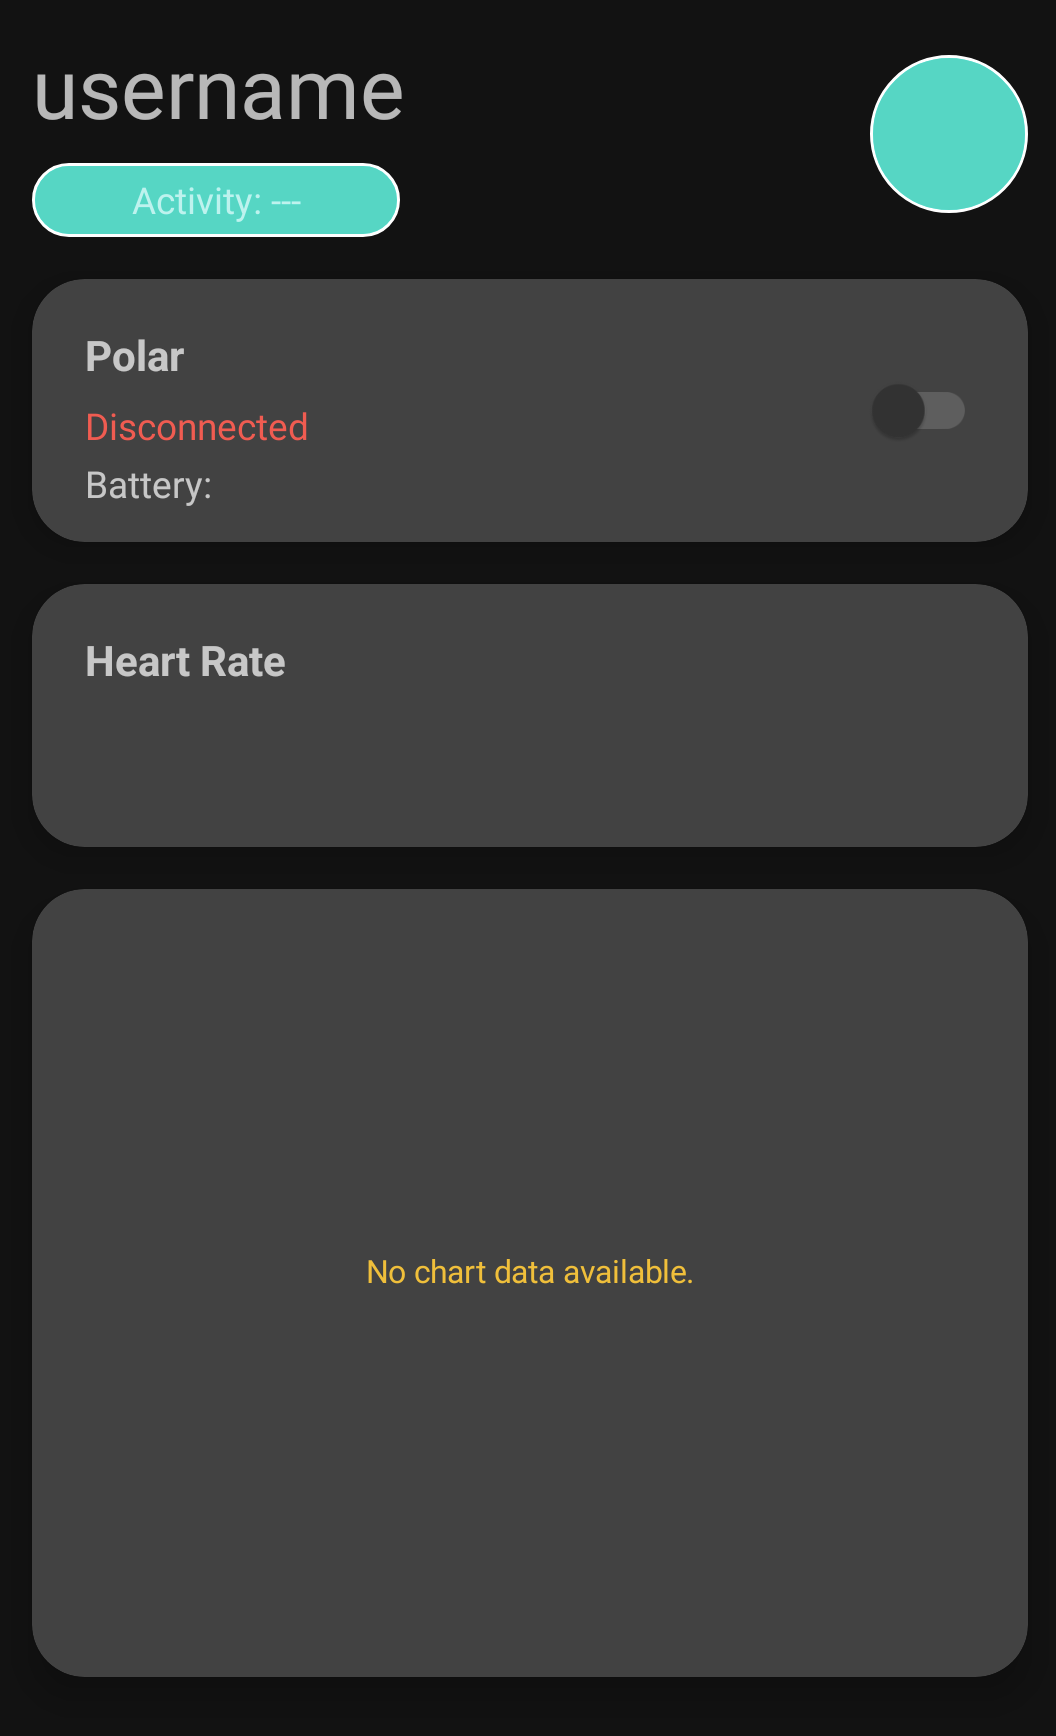
\includegraphics[width=0.4\textwidth]{images/homefragment-screenshot.png}
    \caption{Screenshot of HomeFragment}
    \label{fig:homefragment_screenshot}
\end{figure}

\subsection{ExerciseFragment}
The \texttt{ExerciseFragment} shows an overview of an ongoing exercise. It uses \texttt{DataBinding} to display the exercise details and observing the \texttt{currentExercise} LiveData from the \texttt{ExerciseViewModel}. 
\begin{lstlisting}[caption={Observer for currentExercise (HomeFragment)}]
private fun observeAndUpdateExercise() {
    exerciseViewModel.currentExercise.observe(viewLifecycleOwner) { newExercise ->
        binding.includeExerciseStart.exercise = newExercise
    }
}
\end{lstlisting}

The \texttt{ExerciseFragment} also offers buttons to start and stop an exercise session.
Once the user presses the button to start an exercise session and the process is successfully started, the start button will be automatically disabled to prevent multiple start requests. Similarly, when the stop button is pressed, the stop button will also be disabled to avoid any unintended interruptions. 
This approach ensures that the exercise can be performed without any conflicting or overlapping commands.
To ensure accurate data, the \texttt{ExerciseFragment} observes the current active user and adjusts the exercise information accordingly.

Additionally, a separate fragment called \texttt{ExerciseListFragment} is created inside the \texttt{ExerciseFragment} to display a list of completed exercises. The \texttt{ExerciseFragment} observes \texttt{currentExerciseList} live data from the \texttt{ExerciseViewModel} to receive updates. 
\texttt{RecyclerView}\footnote{\url{RecyclerView} is widget used for displaying sets of data efficiently. URL: \url{https://developer.android.com/reference/androidx/recyclerview/widget/RecyclerView}} widget is used to dynamically display the \texttt{currentExerciseList}. 
\begin{lstlisting}[caption={Observer for currentExercise (HomeFragment)}]
private fun observeExerciseList() {
    exerciseViewModel.currentExercisesList.observe(viewLifecycleOwner) { newExercisesList ->
        initRecyclerView(newExercisesList)
    }
}
\end{lstlisting}
\begin{figure}[H]
    \centering
    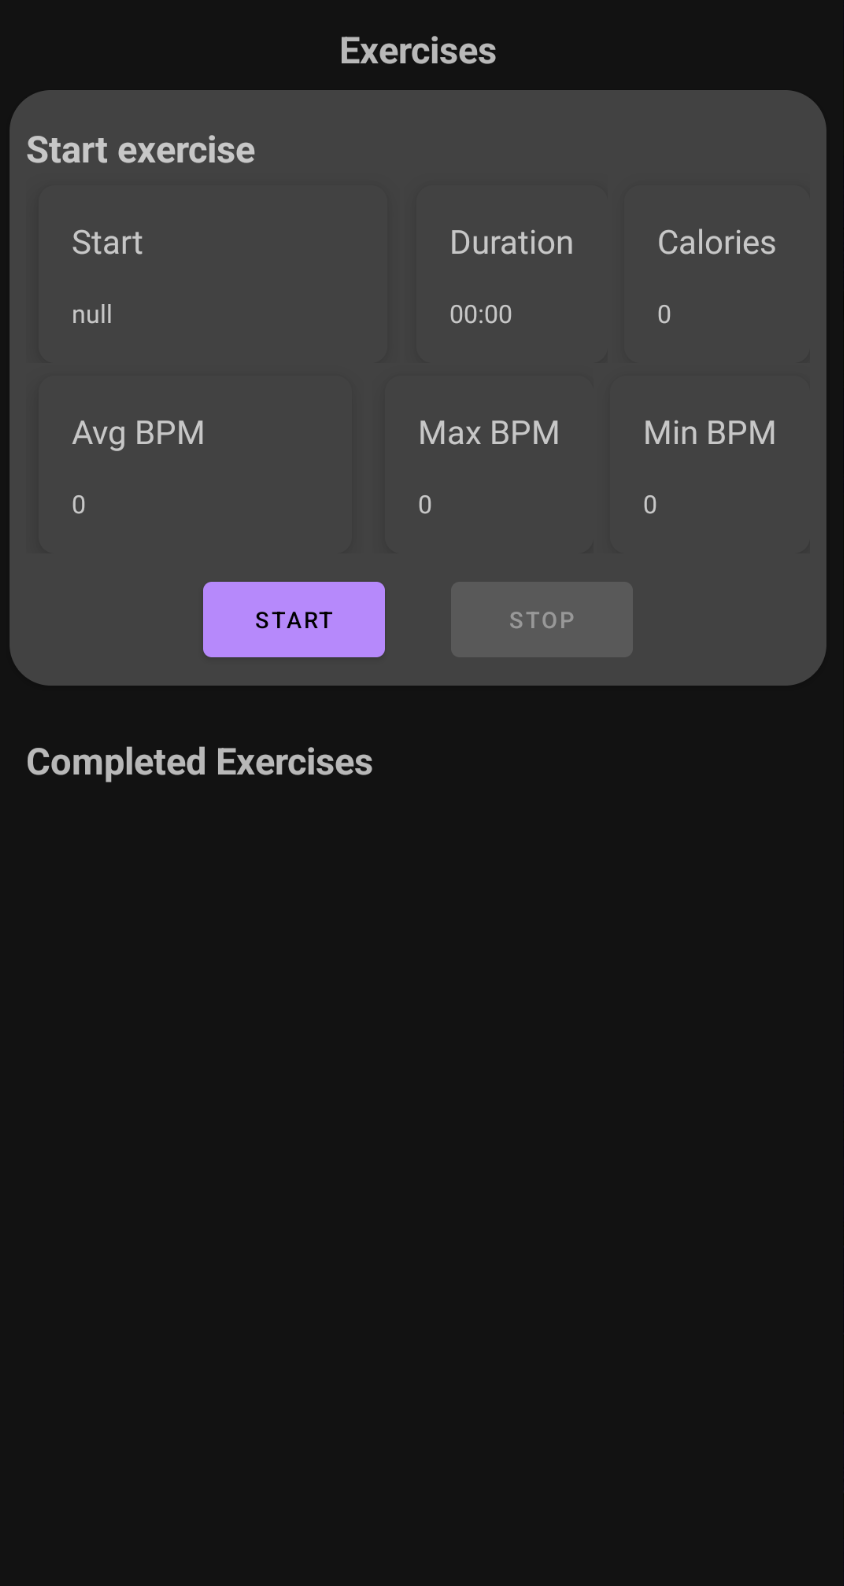
\includegraphics[width=0.5\textwidth]{images/exercisefragment-screenshot.png}
    \caption{Screenshot of ExerciseFragment}
    \label{fig:userfragment_screenshot}
\end{figure}

\subsection{UserFragment}
The \texttt{UserFragment} is responsible for displaying the details of the current active user. 
To achieve this functionality, it observes the \texttt{currentUser} LiveData from the \texttt{UserViewModel} and bind it using \texttt{DataBinding}. 
\begin{lstlisting}[caption={Observer for currentUser (UserFragment)}]
private fun observeActiveUser() {
    userViewModel.activeUser.observe(viewLifecycleOwner) { user ->
        binding.activeUser = user
    }
}
\end{lstlisting}
The user information is displayed in text fields and a calendar is available to support adding or editing the date of birth. 
Additionally, \texttt{UserFragment} provides three buttons for deleting, adding, and updating user data.
\begin{figure}[H]
    \centering
    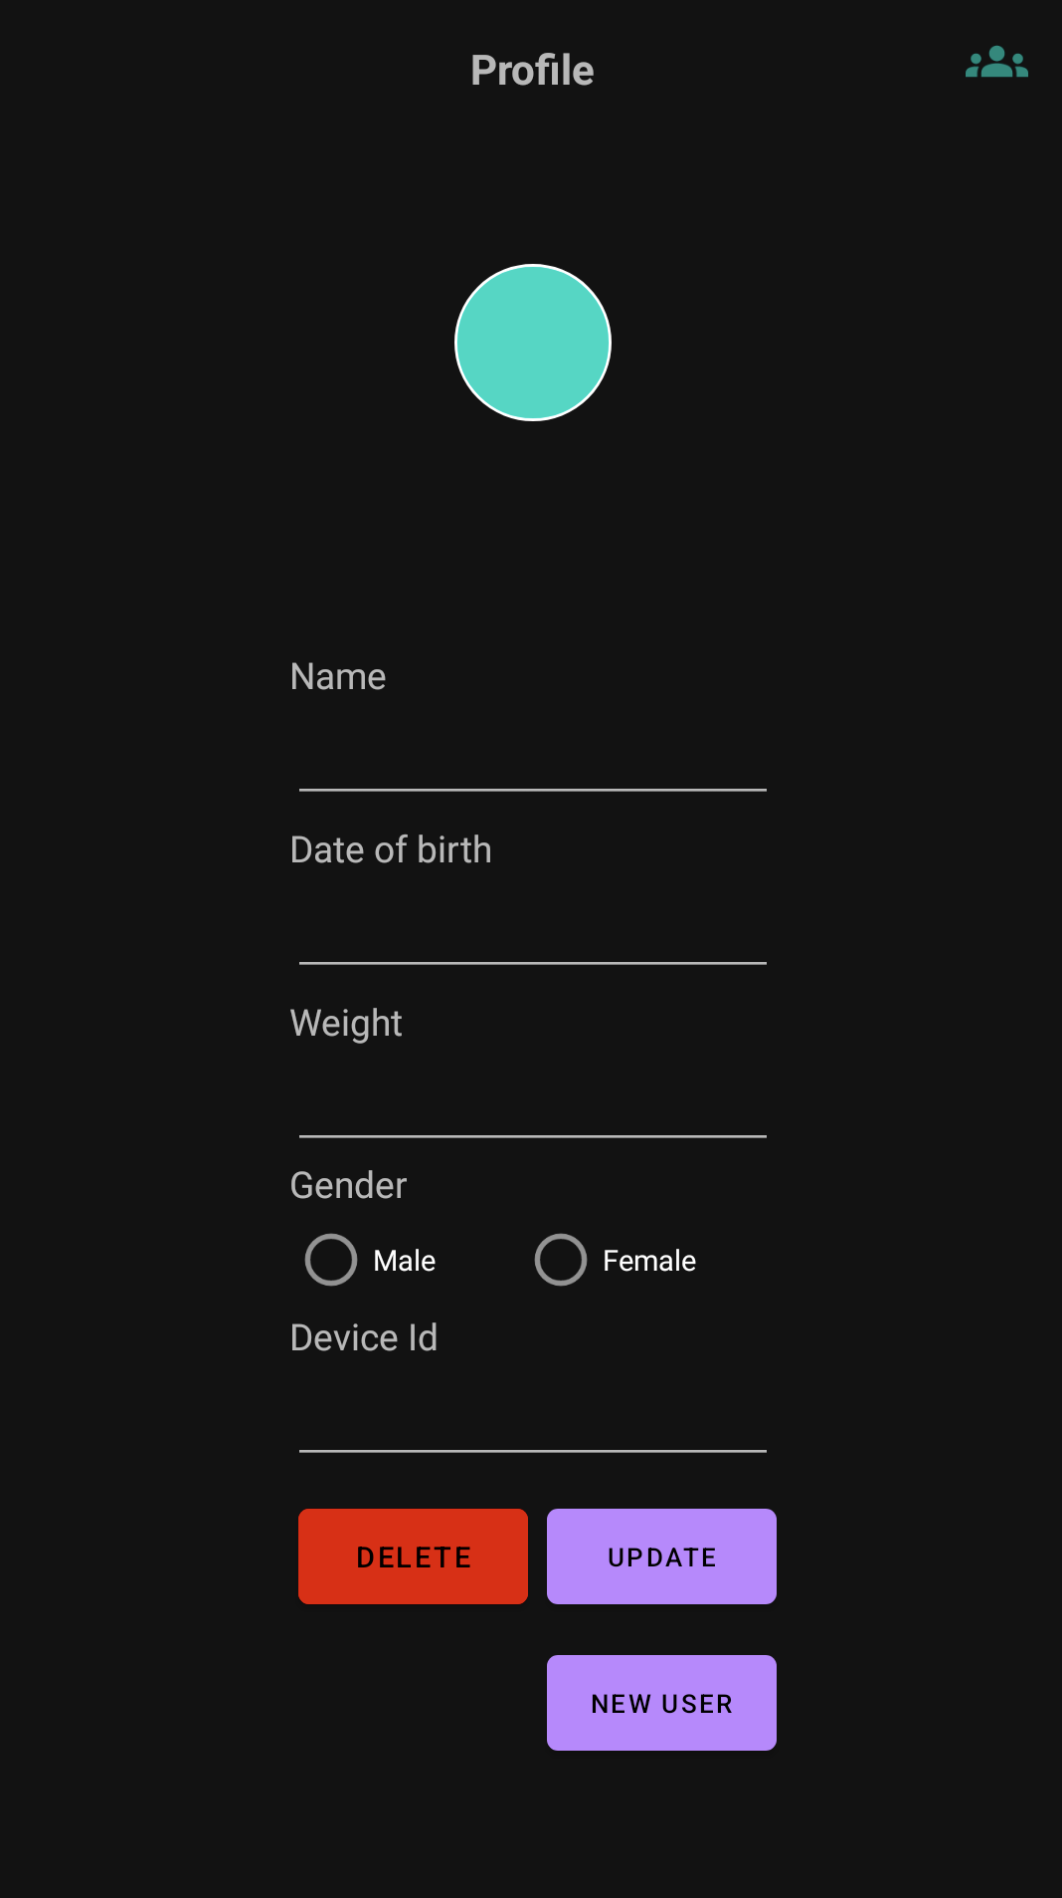
\includegraphics[width=0.5\textwidth]{images/userfragment-screenshot.png}
    \caption{Screenshot of UserFragment}
    \label{fig:userfragment_screenshot}
\end{figure}

Furthermore, a separate \texttt{UserListFragment} is implemented to display a list of all users in the system. 
Similar to the \texttt{ExerciseListFragment}, it uses a \texttt{RecyclerView} to display a list of users. 
Each user in the list is clickable, allowing the user to change the active user by selecting a different user from the list.






\chapter{Evaluation}

The evaluation chapter focuses on demonstrating and evaluating the system based on the defined use cases and quality standards mentioned in \autoref{chap:requirements}. 
The main objective is to assess the system's performance, usability, and compliance to the expected standards. 

\section{Demonstration}
In this section, the application as the result of this thesis will be demonstrated. The demonstration will follow the following procedure to show the key features and functionalities.

Firstly, explore the user management functionality within the application. 
In order for the application to function properly, an active user needs to be created.
To create a new user, simply fill in all the required information in the provided input fields and press on the "New User" button.
Once a user is created, it will be automatically set as the current active user.
To update the information, modify the input fields and press the "Update User" button.
Additionally, the option to permanently delete a user profile is available.
\begin{figure}[H]
    \centering
    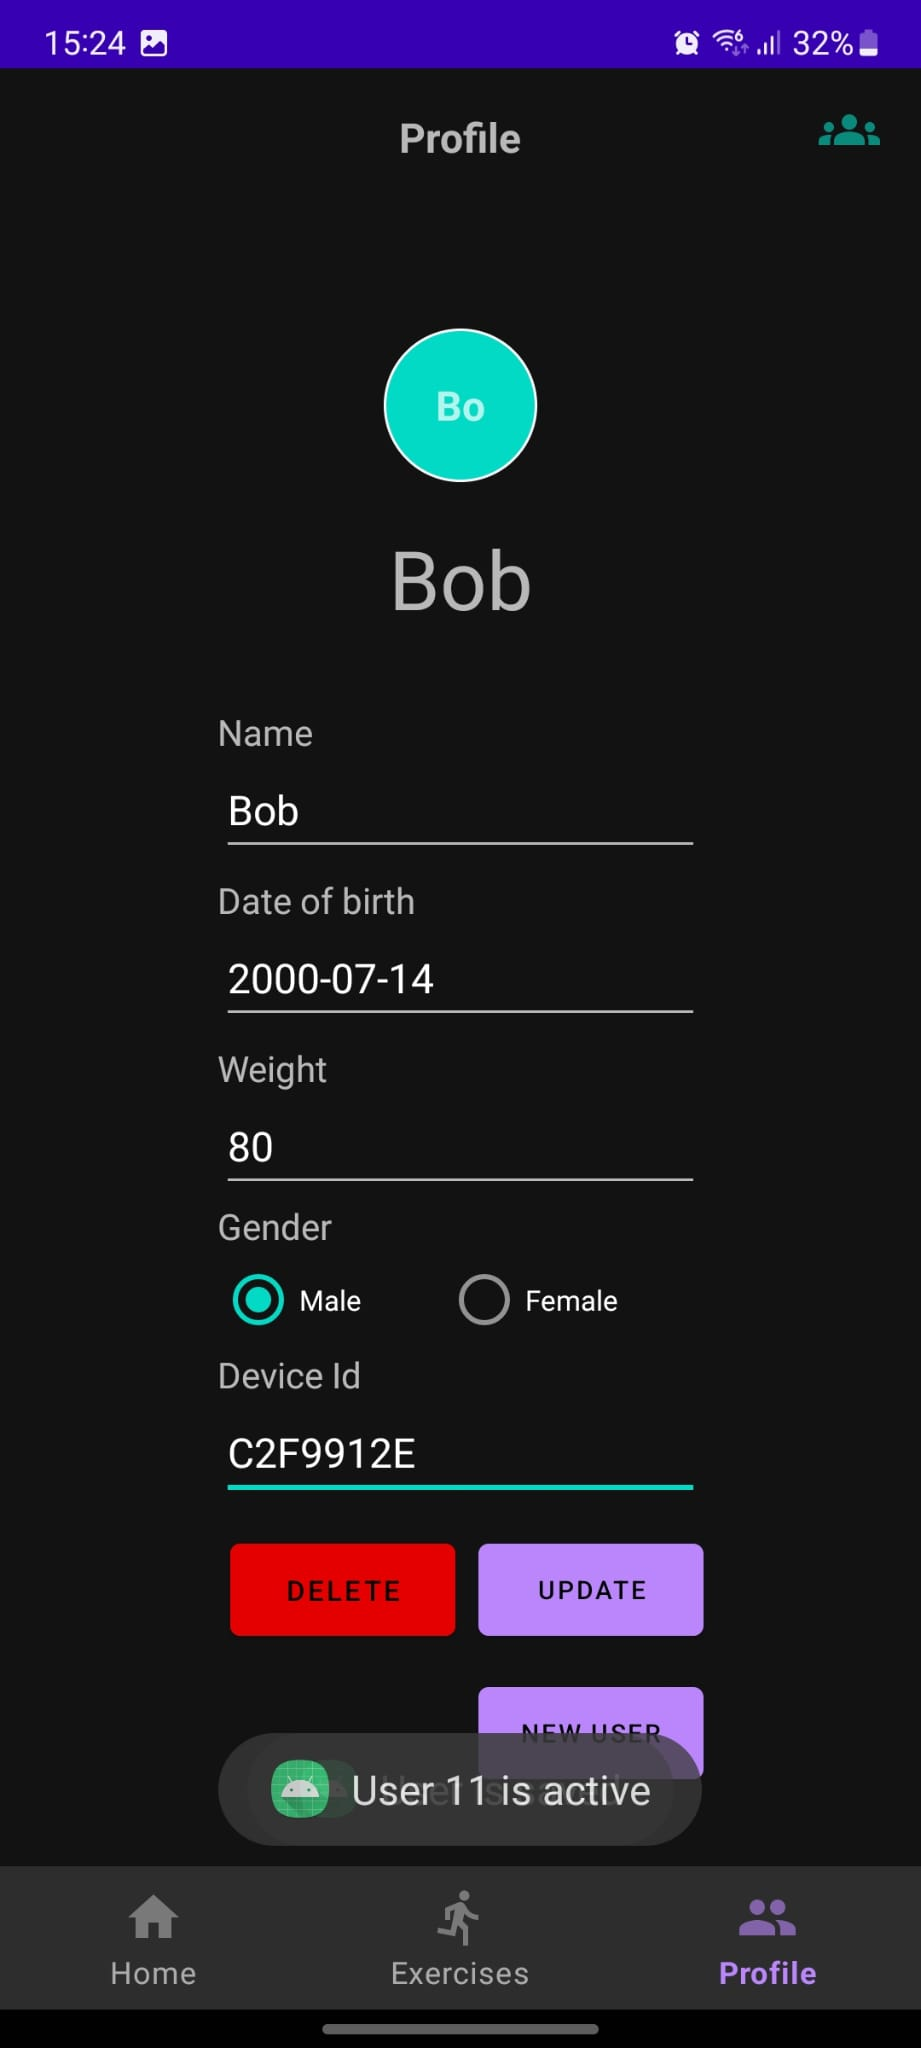
\includegraphics[width=0.5\textwidth]{images/add-new-user.jpeg}
    \caption{Screenshot of successfully adding a new user}
    \label{fig:add-new-user-screenshot}
\end{figure}

Once a user has been successfully added and set active, a connection to the heart rate sensor can be established and heart rate streaming can be started.
Using the bottom navigation, navigate to the home and initiate connection and start heart rate streaming, by simply toggle the switch. 
As the heart rate data is streamed, a dynamic graph will be displayed, providing a visual representation of the user's heart rate.
Furthermore, the user's activity intensity level will be displayed.
\begin{figure}[H]
    \centering
    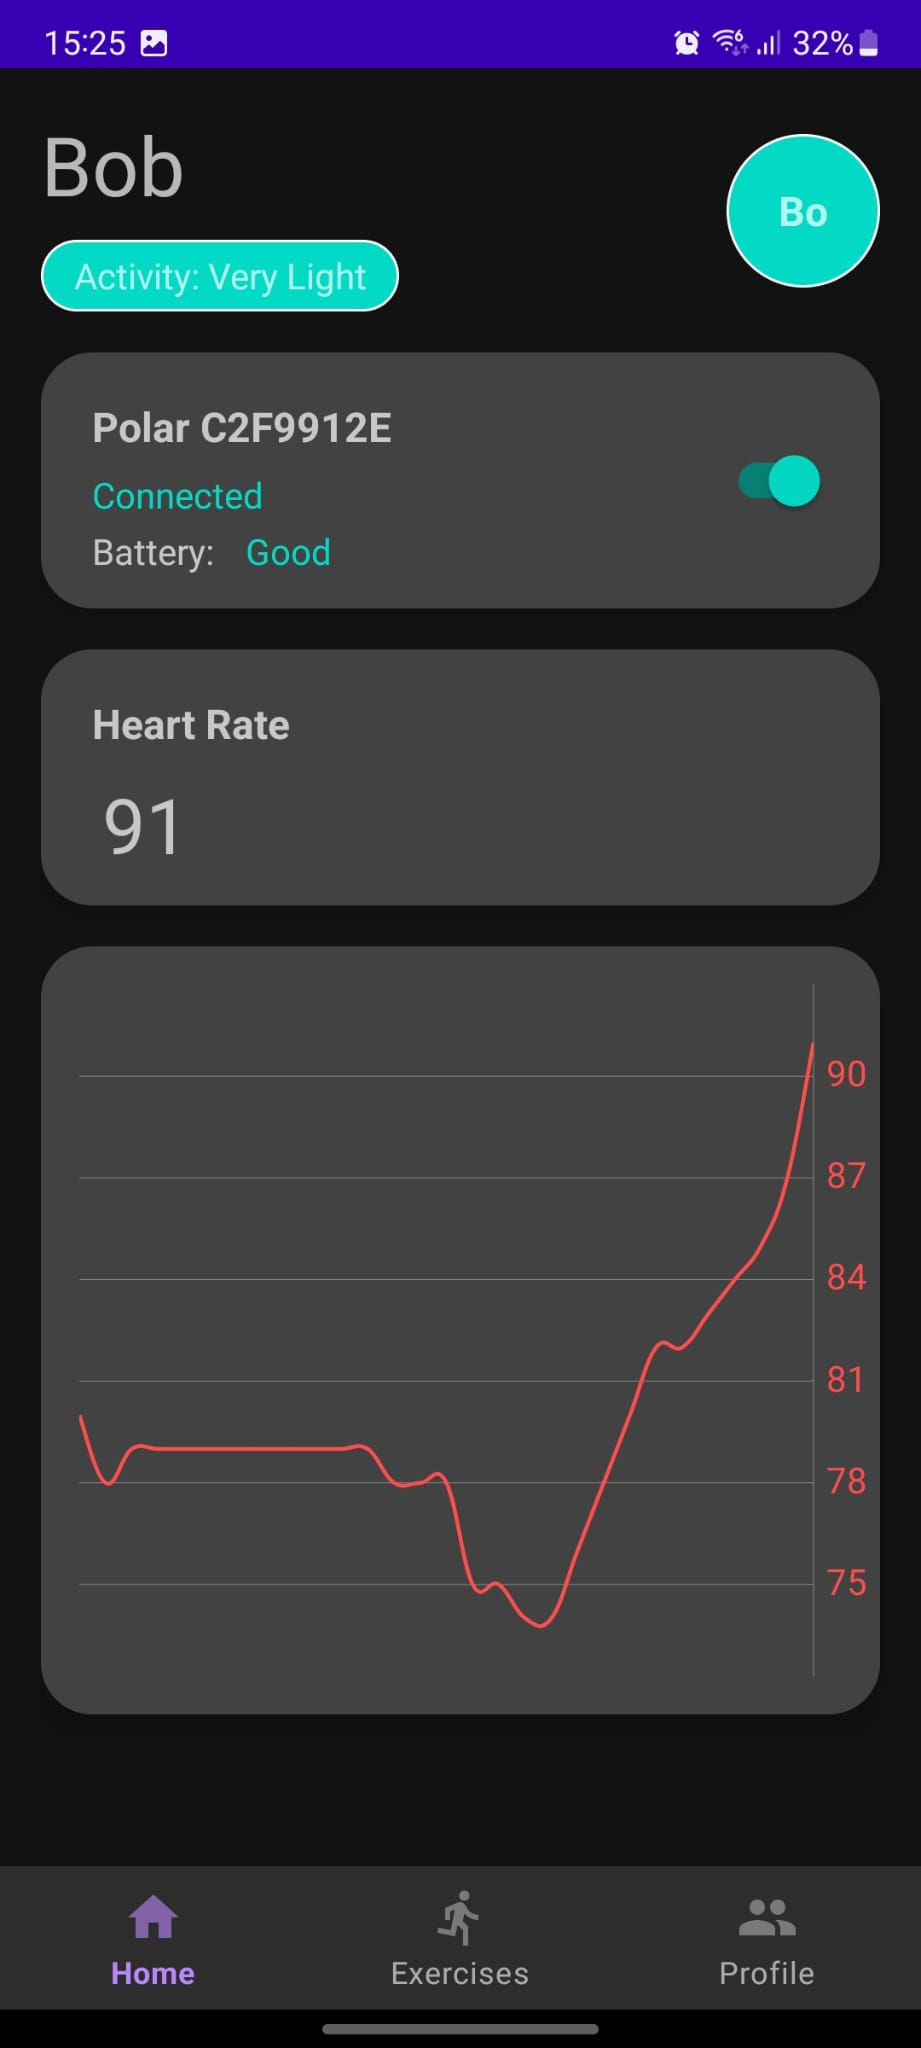
\includegraphics[width=0.5\textwidth]{images/home-sc.jpeg}
    \caption{Screenshot of home page, displaying user's heart rate and activity level}
    \label{fig:home_screenshot}
\end{figure}

After the heart rate streaming has begun, an exercise can be started by navigating to the exercise page and pressing the start button.
The application will then track the exercise progress, including calculating the calories burned. 
To stop the exercise, simply press the stop button. Once an exercise is completed, it will be displayed as shown in \autoref{fig:exercise_screenshot}, providing a record of the user's workout history.
\begin{figure}[H]
    \centering
    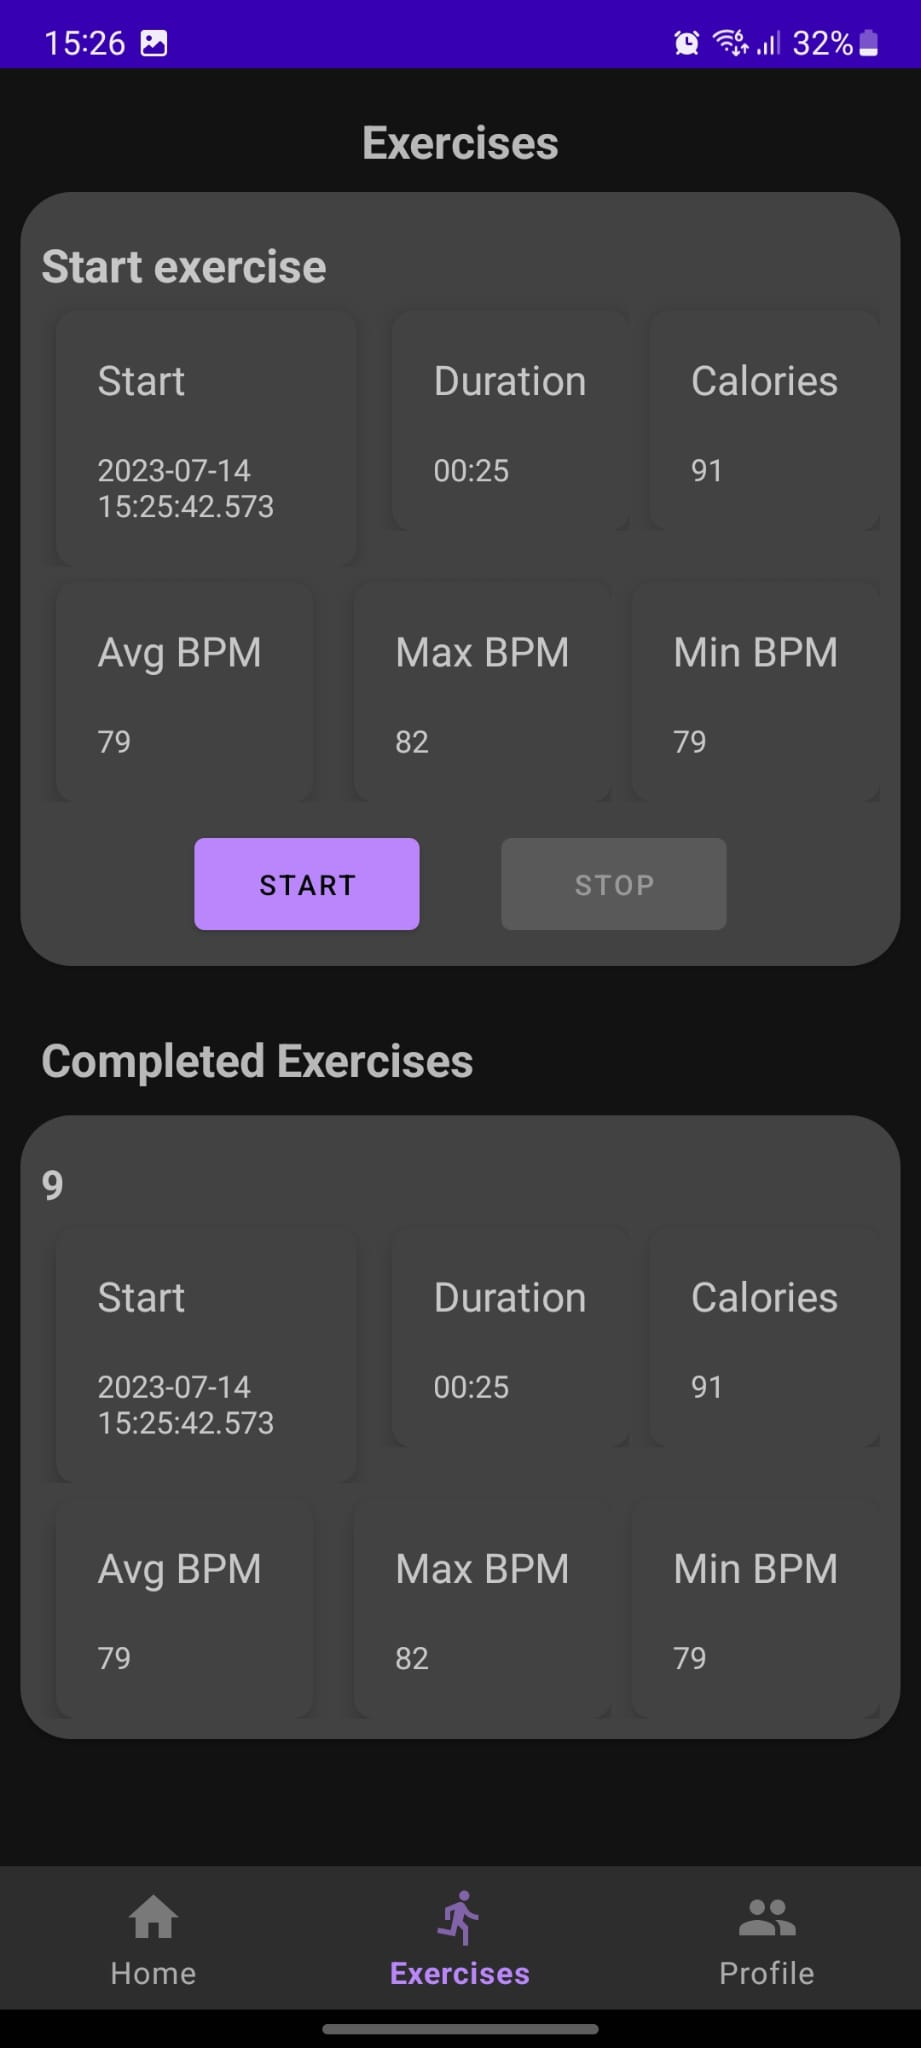
\includegraphics[width=0.5\textwidth]{images/exercise-tracking-sc.jpeg}
    \caption{Screenshot of exercise page, displaying user's exercise information}
    \label{fig:exercise_screenshot}
\end{figure}

\section{Evaluation}
The fulfillment of the requirements and standards outlined in \autoref{chap:requirements} should be used as an assessment metric to determine if the system and its functions have achieved their primary purpose in alignment with the goals of this thesis. 
The implementation of each user story detailed in \autoref{chap:use_case} is listed in \autoref{tab:user_story_and_assessment}.
\clearpage
\begin{longtable}{p{0.5\textwidth} p{0.5\textwidth}}
    \label{tab:user_story_and_assessment}\\

    \caption{Implementation of the user stories}\\
        \hline
        \textbf{User Story} & \textbf{Implementation} \\
        \hline
        As a health-oriented user, I want to monitor my cardiovascular activity so that I can stay informed about my physical wellbeing. & Provides a functionality to control connection to the heart rate sensor and start heart rate data streaming. The received heart rate data is visualized in form of a line graph.\\
        \hline
        As a physically active individuals, I want to track my current activity so that I can make adjustments to my physical activities. & Processes the received heart rate data to show the intensity of the user's current activity and displays it on the user interface.\\    
        \hline
        As a fitness enthusiast, I want to know the number of calories burned in my exercises. This allows me to keep track of my progress and make adjustments to my exercises. & Provides a functionality to start and stop user's exercise and the burned calories will be automatically calculated. The completed exercises are also displayed in the user interface.\\
        \hline
        As a user of the application who is concerned about data privacy, I want full control of my data so that I can manage it easily.  & Provides an interface to add, update, and delete user data.\\
        \hline
\end{longtable}

The implementation of Bluetooth Low Energy to establish connection between the application and the heart rate sensor ensures efficient battery usage while providing real-time streaming of heart rate data. 
The application processes the received heart rate data and transforms it into an interactive line graph. 
However, it would be beneficial to include time information in the graph to provide a clearer understanding of the heart rate history.

Furthermore the application determines the user's physical activity intensity level based on the received heart rate data, allowing the users to monitor their activity intensity level.

Moreover, the exercise tracking feature provides user the ability to track their own exercise. The application displays the duration, heart rate information, time and calories burned during the exercise.
However, the application might not provide the most precise estimation of calories burned during exercises because the formula that is used for the calculation is based on an article published in 2005\autocite{keytel2005energy}.     

From the user management perspective, the application provides users with full control over their own data, allowing them to add, update, and delete their own data.
This feature improves the overall user experience by providing control and ownership over their data.

Additionally, the application should be assessed based on the standards described in \autoref{tab:qualitystandard} to determine the quality of the application.
\newline
\newline
\newline
\begin{longtable}{p{0.2\textwidth} p{0.2\textwidth} p{0.5\textwidth}}
    \label{tab:qualitystandard_evaluation}\\

    \caption{Evaluation of the result application based on the standard described in \autoref{tab:qualitystandard}}\\

        \hline
        \textbf{ID} & \textbf{Relevance} & \textbf{Completion} \\
        \hline
        \multicolumn{3}{@{}l}{\textbf{Navigation}} \\
        VX-N1 & less important & complete, the app supports back button navigation.\\
        VX-N2 & less important & complete, the app supports gesture navigation.\\
        VX-N3 & important & complete, the \emph{fragments} will retrieve data at the start of their lifecycle. \\

        \multicolumn{3}{@{}l}{\textbf{UI and Graphics}} \\
        VX-U1 & less important & incomplete\\
        VX-U3 & less important & incomplete\\
  
        \multicolumn{3}{@{}l}{\textbf{Visual quality}} \\
        VX-V1 & less important & complete, icons are implemented using vector drawables.\\
        VX-V3 & not important & complete, the app supports dark theme using Material Design.\\
        
        \multicolumn{3}{@{}l}{\textbf{Accessibility}} \\
        VX-A1 & less important & incomplete, there are some targets smaller than 48dp\\
        VX-A2 & important & complete, the app display are easily readable.\\
        
        \multicolumn{3}{@{}l}{\textbf{Background Service}} \\
        FN-B1 & important & complete, there are restriction for \texttt{ExerciseService} and \texttt{ConnectionService}. Only one instance of each services can run at the same time.\\

        \multicolumn{3}{@{}l}{\textbf{Stability}} \\
        PS-S1 & very important & complete, the application does database transactions in a coroutine.\\

        \multicolumn{3}{@{}l}{\textbf{Performance}} \\
        PS-P1 & important & incomplete\\
        
        \multicolumn{3}{@{}l}{\textbf{Permissions}} \\
        SC-P1 & important & complete.\\
        SC-P4 &  important & complete, at the first time the app starts, permissions are asked and explained the usage. \\
        SC-P5 & important & incomplete\\
        
        \multicolumn{3}{@{}l}{\textbf{Data \& Files}} \\
        SC-DF1 & important & complete, all of the data are stored in local database.\\
        SC-DF2 & important & complete, logging only contains the id of the entities.\\
        SC-DF3 & not important & complete.\\

        \hline
\end{longtable}
\chapter{Conclusion}


\section{Summary}

\section{Reflection}
demo
things to improve

\section{Evaluation}



%----------------------------------------------------------------------------------------
%	REFERENCE LIST
%----------------------------------------------------------------------------------------

\printbibliography[
heading=bibintoc,
title={Bibliography}
]


\newpage
\chapter{List of Abbreviation}

\begin{longtable}{p{0.2\textwidth} p{0.8\textwidth}}
    ANR & Android Not Responding \\
    APP & Application \\
    BLE & Bluetooth Low Energy \\
    BPM & Beats Per Minute \\
    CI/CD & Continuous Integration Continuous Development \\
    CRUD & Create, Read, Update and Delete \\
    DB & Database \\
    HR & Heart Rate \\
    IDE & Integrated Development Environment \\
    IMEI & International Mobile Equipment Identity \\
    ISM & Industrial, Scientific, and Medical \\
    MVVM & Model-View-ViewModel \\
    SDK & Software Development Kit \\
    UI & User Interface \\
    XML & Extensive Markup Language \\

\end{longtable}
\newpage

\appendix

\pagenumbering{Roman}

\chapter{Appendix}


\section{Source Code}
\begin{lstlisting}[caption={Implementation of EventBus (Kotlin - HeartrateEventBus)}]
object HeartrateEventBus {
    private val listeners = mutableListOf<(HeartrateEvent) -> Unit>()

    fun subscribe(listener: (HeartrateEvent) -> Unit) {
        listeners.add(listener)
    }

    fun unsubscribe(listener: (HeartrateEvent) -> Unit) {
        listeners.remove(listener)
    }

    fun publish(event: HeartrateEvent) {
        listeners.forEach { listener ->
            listener.invoke(event)
        }
    }
}
\end{lstlisting}

\begin{lstlisting}[caption={Implementation of calorie calculation (Kotlin - ExerciseService)}]
private fun calculateCalories(exercise: Exercise): Float {
    return if (user.gender == Gender.MALE) {
        (exercise.duration * (0.6309*exercise.averageHrBpm!! + 0.1988*user.weight + 0.2017*user.getAge() - 55.0969) / 4.184).toFloat()
    } else {
        (exercise.duration * (0.4472*exercise.averageHrBpm!! + 0.1236*user.weight + 0.074*user.getAge() - 20.422) / 4.184).toFloat()
    }
}
\end{lstlisting}

\section{Supplemental Figures}
\begin{figure}[H]
    \centering
    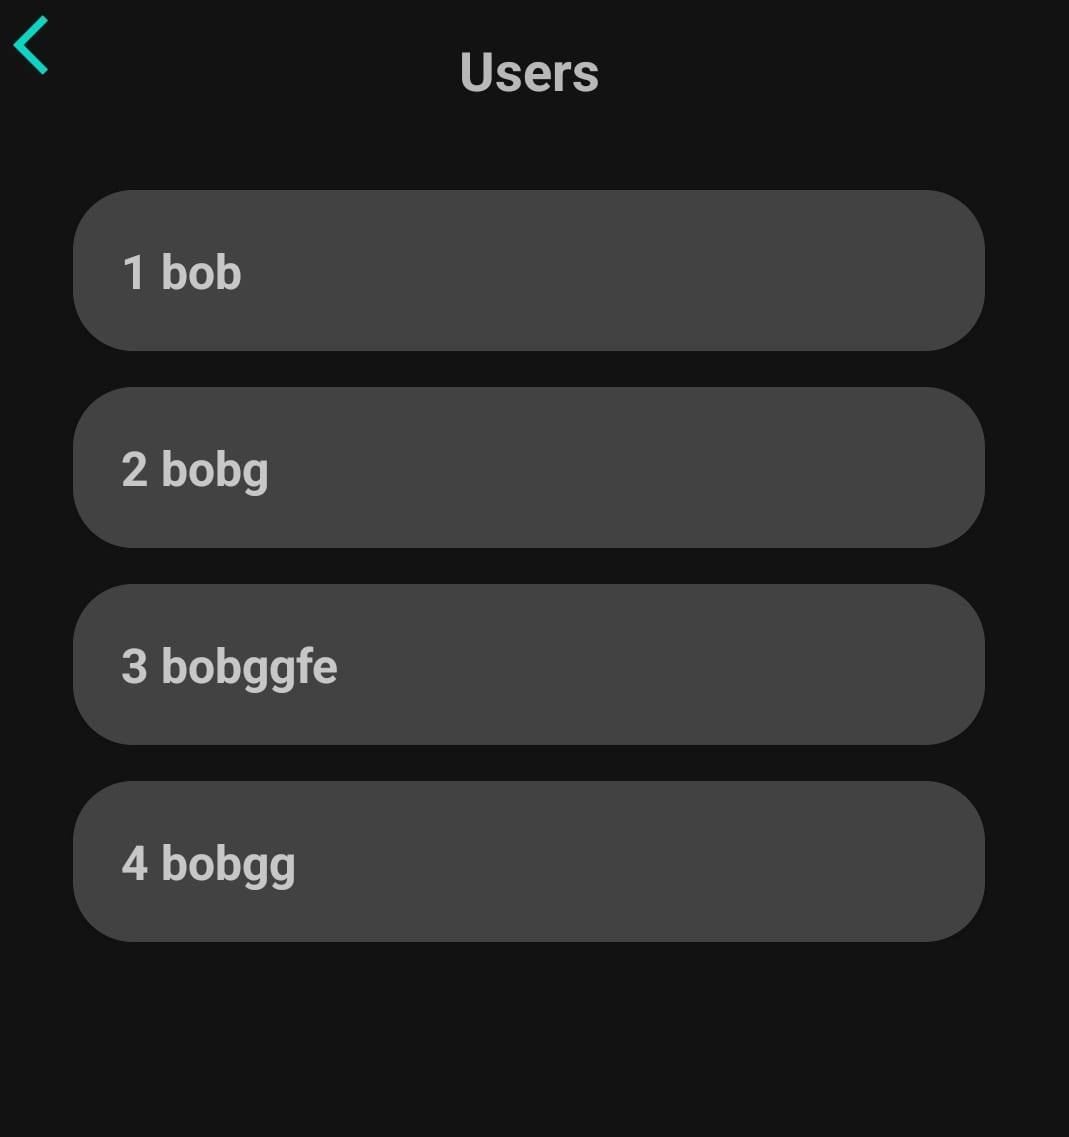
\includegraphics[width=0.7\textwidth]{images/userlistfragment-screenshot.jpeg}
    \caption{Screenshot of UserListFragment containing all users}
    \label{fig:userlistfragment}
\end{figure}


\newpage
\thispagestyle{empty}       % keine Seitennummer
\noindent

\section*{Eidesstattliche Versicherung}
Hiermit versichere ich an Eides statt durch meine Unterschrift, dass ich die vorstehende Arbeit selbstst\"andig und ohne fremde Hilfe angefertigt und alle Stellen, die ich w\"ortlich oder ann\"ahernd w\"ortlich aus Ver\"offentlichungen entnommen habe, als solche kenntlich gemacht habe, mich auch keiner anderen als der angegebenen Literatur oder sonstiger Hilfsmittel bedient habe. Die Arbeit hat in dieser oder \"ahnlicher Form noch keiner anderen Pr\"ufungsbeh\"orde vorgelegen.\\
\linebreak[4]
\linebreak[4]
\linebreak[4]
\linebreak[4]
-------------------------------------------------------\linebreak[4]
Datum, Ort, Unterschrift



\end{document}

